\documentclass[a4paper,12pt,titlepage]{report}
\linespread{1.3}
\usepackage{setspace}
\onehalfspacing 

% NOTE -> Changed to remove natbib data error in compilation
\usepackage[square,sort,comma,numbers]{natbib}
%\usepackage{natbib}
\usepackage{makeidx}
\usepackage{graphicx}
\usepackage{ccaption}
%\usepackage{subfigure}
\usepackage{rotating}
\usepackage{lscape}
\usepackage{verbatim}
\usepackage{amsmath, amsthm,amssymb}
\usepackage{mathrsfs}

% ADDED:
\usepackage{subcaption}
\usepackage{tikz}
\usetikzlibrary{positioning}
\usetikzlibrary{shapes.geometric, arrows}
\usepackage{hyperref}
\usepackage[section]{placeins}
\usepackage[final]{pdfpages}

% Initial set up for algorithm description:
\tikzstyle{basic} = [rectangle, rounded corners, minimum width=3cm, minimum height=1cm,text centered, draw=black, text width=3cm]
\tikzstyle{io} = [rectangle, rounded corners, minimum width=3cm, minimum height=1cm, text centered, draw=black, text width=3cm, line width=0.5mm,font=\bf]
\tikzstyle{main} = [rectangle, rounded corners, minimum width=3cm, minimum height=1cm, text centered, draw=black, text width=3cm, font=\bf]
\tikzstyle{main_long} = [rectangle, rounded corners, minimum width=6cm, minimum height=1cm, text centered, draw=black, text width=6cm, font=\bf]
\tikzstyle{temp} = [rectangle, rounded corners, dashed, minimum width=6cm, minimum height=1cm, text centered, draw=black, text width=6cm, font=\bf]

\tikzstyle{wls} = [black,thick]
\tikzstyle{uwsg} = [blue,thick]
\tikzstyle{posg} = [red,thick]
\tikzstyle{wfd} = [cyan,thick]
\tikzstyle{uwfd} = [green,thick]
\tikzstyle{fdsm} = [magenta]

\newtheorem{theorem}{Theorem}[section]
\newtheorem{lemma}[theorem]{Lemma}
\theoremstyle{definition}\newtheorem{definition}[theorem]{Definition}
\newtheorem{proposition}[theorem]{Proposition}
\newtheorem{corollary}[theorem]{Corollary}
\newtheorem{example}{Example}
\theoremstyle{remark}\newtheorem*{remark}{Remark}

\newcommand{\Phid}[0]{\dot{\Phi}}
\newcommand{\Phib}[0]{\bar{\Phi}}

\newcommand{\de}[0]{\delta}
\newcommand{\deb}[0]{\bar{\delta}}

\newcommand{\that}[0]{\hat{\theta}}

%\usepackage{endfloat}
%\nomarkersintext
\pagestyle{plain}
\topmargin -0.6true in
\textwidth 15true cm
\textheight 9.5true in
\oddsidemargin 0.25true in
\evensidemargin 0.25true in
\headsep 0.4true in

\usepackage{fancyheadings}
\pagestyle{fancy}
\addtolength{\headheight}{2.5pt}
\renewcommand{\chaptermark}[1]{\markboth{\thechapter~~#1}{}}
\renewcommand{\sectionmark}[1]{\markright{\thesection~~#1}{}}
\ifthenelse{\boolean{@twoside}}
{
        \rhead[\bfseries \rightmark]{\bfseries \thepage}
        \lhead[\bfseries \leftmark]{\bfseries \thepage}
        \addtolength{\headwidth}{\marginparsep}
        \addtolength{\headwidth}{\marginparwidth}
}{
        \lhead{\bfseries \leftmark}
        \rhead{\bfseries \thepage}
}
\cfoot{}

%---------------------------------------------------------
%---------------------------------------------------------
\begin{document}

\begin{titlepage}
\title{Improving strain estimation methods in compression optical coherence elastography towards intra-operative imaging.}
\author{Emily Hackett \\
{{\it Supervisors:} Dr Brendan Kennedy and Dr Lixin Chin}\\
{Honours Thesis submitted as part of the B.Phil. (Honours) degree} \\ {in the School of Physics, University of Western Australia}\\ \\}
\date{Date of submission: 04/11/17}
\maketitle
\end{titlepage}


               % This is who you are

\newpage

%\chapter*{Declaration}
%\thispagestyle{empty}
%{I declare that this thesis contains less than 15 000 words}
%\\
%\\
%\\
%\\
%Joe Citizen
%\newpage
\chapter*{Acknowledgments}
\thispagestyle{empty}

I'd like to thank my supervisors, Dr Brendan Kennedy and Dr Lixin Chin, for their unwavering support and enthusiasm for the project, as well as their wealth of interesting suggestions for the project. 

I would also like to thank Dr Philip Wijesinghe, who was extremely helpful in providing insight to different processing techniques, and aiding in the inevitable debugging.

To Matt Hepburn, for his previous work on strain estimation techniques and image analysis, without which this project wouldn't nearly have gotten so far. Also for generously allowing use of his data sets. 

To the BRITELab research group at Harry Perkins, for being such a welcoming community. 

Lastly to the staff at the School of Physics UWA, in particular Ian McArthur and Darren Grasso, for their continued support throughout my undergraduate degree, as well as the enthusiasm they have inspired in their students for the broad range of areas on which physics can shed light.
   % This is who you thank

\newpage

\begin{abstract}

	In WA, re-excision rates for breast conserving surgery were estimated to be 30\% in 2017, due to inaccurate detection of tumour margins during surgery. There is a need for fast imaging techniques capable of assessing tumour margins in breast tissue with high resolution and within intra-operative time frames. Cancer often causes changes in the mechanical properties of tissue, with tumour masses often reported to be stiffer than surrounding healthy tissue.
	Elastography describes a family of imaging techniques capable of imaging these changes in mechanical properties by examining their response to mechanical loading. \ac{oce} refers to a number of elastography techniques that utilise \ac{oct} as the underlying imaging technique, and are therefore capable of producing images of mechanical properties (such as stiffness, or strain response), on the micrometre resolution scale, with mm to cm field of view size, however only at shallow (mm) penetration depths. To make use of \ac{oce} in intra-operative surgical margin assessment for breast cancer, there is a need to produce images of strain rapidly. In order to do this, fast strain estimation algorithms must be developed, that maintain high image quality in terms of sensitivity and image resolution. 
	
	Six strain estimation algorithms, differentiated by their phase unwrapping technique and the strain differentiation filter applied, are implemented and analysed on a silicon phantom, using the metrics of processing time, strain sensitivity and image resolution. It was found that strain estimation techniques utilising Gaussian smoothing with finite difference were the fastest, and had similar sensitivity to other techniques. Applying lateral averaging on top of the strain estimation further increased the sensitivity, however at the cost of axial and lateral image resolution. 

	It was found that using an unweighted Gaussian filter on the phase difference, followed by finite difference, produced the optimum combination of processing speed, sensitivity and image resolution. Further work is suggested in terms of implementing the algorithms in parallel, possibly on \ac{gpu}s, and further extension into quantitative elastography.
	
\end{abstract}


          % This is your thesis abstract

\pagenumbering{roman}
\newpage
%---------------------------------------------------------
% Do the table of Contents and lists of figures and tables
%---------------------------------------------------------
\tableofcontents
\markboth{}{}
\newpage

\pagenumbering{arabic}
%---------------------------------------------------------
%---------------------------------------------------------
%Include the chapters!

\chapter{Introduction}

\section{Boundary Detection in Breast-Conserving Surgery}
%!! IMPORTANCE OF ACCURATE BOUNDARY DETECTION IN BREAST-CONSERVING SURGERY !!
% provide motivation towards real-time imaging & project significance

\section{Clinical Significance}

Once such area for real-time surgery application of OCE is in breast cancer surgery. (... Details about current diagnosis techniques in breast cancer surgery ...) Having a surgical tool capable of real-time in vivo imaging of excised tissue boundaries has the potential to reduce the re-excision rates in breast cancer patients.

To be able to provide real-time OCE images in surgery, the processing of the optical data from the OCT system to produce elastography images must be done in real-time also. One way to speed up the processing is to remove the need for quantitative analysis, and use qualitative only, that is, focus on the detectable difference between healthy and cancerous tissue using qualitative images. Standard OCE elastograms (elastography images), combine measurements of strain and stress to produce quantitative maps of tissue elasticity. However, to produce qualitative images of tissue mechanical properties, that differentiate softer from stiffer objects (such as healthy stroma from tumour), requires only images of strain. 

\section{Elastography}
Elastography uses the application of an external mechanical load on a tissue to produce images of mechanical contrast. These maps of mechanical properties of tissue offer insight into the study of disease at scales varying from organs to tissue microarchitecture, which can be probed by utilising different imaging techniques to investigate the deformation of the tissue. Most elastography techniques utilise the assumption that tissue is a linearly elastic solid \cite{kennedy_review_2014}, an assumption that is valid for applications of small mechanical loads, and that greatly simplifies elastogram processing. 

Optical coherence elastography (OCE) is a medical imaging tool used to examine the mechanical properties of tissue. The underlying imaging technique, optical coherence tomography (OCT), relies on the optical properties of tissue to generate contrast in an image formed by backscattered light. Elastography produces images of the stiffness, or elasticity, of a tissue. The sense of touch used by a surgeon to differentiate stiff tumour from softer healthy tissue is analogous to elastography on a much coarser scale, however elastography has the potential to enable quantitative images of mechanical properties of tissue to be formed. The use of OCT as the underlying imaging tool for elastography also allows much higher resolution imaging, providing access to the mechanical properties of tissues on the micrometre scale. 

The significance of OCE lies in its ability to provide high resolution images at low sample depths. These properties differentiate it from other techniques, such as ultrasound elastography, which could be used to image deep within the body due to the higher penetration of sound waves into tissue. The ideal application of OCE is at surface tissue (such as imaging the retina, or skin), on excised tissue in a surgical setting, or used as a tool during surgery on uncovered tissue. The third application forms the main motive for this project.

\section{Project Aims}

The current processing algorithm used by the BRITELab group to process strain on a bench top OCE system can scan a 3D volume in about (??). In order to process strain in real-time, this must be sped up by a factor of (??). The purpose of this thesis is to investigate techniques of speeding up the processing of strain in OCE, for the purpose of real-time surgical application in breast cancer surgery. The goal is to compare strain estimation techniques on a simulated phantom using metrics of processing time (as an indication of its ability to be extended to real-time surgical application) and sensitivity (to monitor image quality). Once the strain estimation technique has been narrowed down to a small selection of optimal methods, the resulting image resolution is investigated as a measure of the ability to detect object boundaries in strain elastograms. Finally, these final selected methods are tested on a sample excised breast data set to investigate how the image quality prevails in realistic data.
           
\chapter{The Physics of OCE}

OCE can be thought of as the combination of a foundational imaging technique, optical coherence tomography, and its application to imaging mechanical properties: elastography. These two pillars of OCE are examined first separately, in Sections 2.1 and 2.2, then as connected components of a composite OCE system in Section 2.3. In this section, the characteristics of standard OCE systems are discussed, with an eye to understanding the implications of the phase-sensitive, compression OCE system used in this project.

\section{Optical Coherence Tomography}
Optical coherence tomography (OCT) can be thought of as the optical equivalent to ultrasound, in that it detects the light reflected from scatterers within a tissue. The reflected light interferes with a reference beam, enabling depth-resolved reconstruction of the location of the scatterers within the sample \cite{chin_parametric_2016}. Because the speed of light in tissue is significantly higher than that of sound, OCT offers a much higher resolution than ultrasound, on the order of $5-15 \mu m$ \cite{kennedy_emergence_2017}, as limited by the coherence length of the light source \cite{huang_optical_1991}. However, this higher resolution comes at the expense of depth of penetration into the tissue, which for OCT, is only $1-2mm$ beneath the surface \cite{schmitt_optical_1999}, in comparison to the relatively deep imaging capabilities of ultrasound.

Time-domain OCT uses a simple low coherence Michelson interferometer set up, where the interference signal is measured between the light reflecting from the tissue, and an scanned reference mirror that changes the depth imaged \cite{huang_optical_1991}. The scanning of the reference mirror to image into the tissue produces a 1D A-scan, that contains information about the detected irradiance of the interferometer as a function of depth. Taking multiple A-scans across by moving laterally across a sample surface produces a 2D B-scan. Multiple B-scans can be used as cross-sections to build up an entire 3D scan volume, otherwise known as a C-scan, a process which can be seen in Figure 2. These descriptions are taken from those conventionally utilised in ultrasound imaging. The disadvantage of this set up however is the expensive acquisition times for imaging of 3D volumes.

Fourier-domain OCT systems remove the need for a scanning mirror, and allows the reproduction of a single A-scan with one detection event based on principles of spectral interferometry \cite{chin_parametric_2016}. Rather than detecting the reflected intensity as a function of depth as in time-domain OCT, it is detected as a function of wavenumber of a broadband or swept frequency light source. The Wiener-Khinchin theorem dictates that the inverse Fourier transform of this measured spectral density provides the complex coherence function at different depths along the A-scan line \cite{schmitt_optical_1999}. The speed up using Fourier-domain OCT over time-domain OCT allows the imaging of 3D volumes, of approximately $10mm \times 10mm \times 2mm$ to be acquired in less than 1 second \cite{kennedy_emergence_2017}. The benefit of Fourier-domain OCT over time-domain is not only in allowing a much faster acquisition time, but it also produces a complex signal that carries phase information, allowing it to be used as to quantify displacement within a sample, as described in Section 1.3.

% NOTE -> Try change the topic below, or the title (should not have OCE section in Physics of OCE chapter)
\subsection{Extension to Elastography}
Many elastography methods based on optical imaging techniques exist, and can be differentiated between by examining how the mechanical load is applied to the tissue, as well as what parameter is utilised to form the image, or 'elastogram'. These different factors, as well as the underlying imaging technique, determine the resolution and penetration of the resulting imaging. In addition these parameters may be quantitative or qualitative, which has implications for diagnostic capability, and mechanical loading methods can be simple or complex, which introduces limitations on image acquisition time.

Elastography techniques commonly used with optical imaging modalities, among others, can be thought of in three categories: compressive, resonant and shear wave based elastography. Static or quasi-static methods of loading include compressing the tissue, either through an indentation point or in bulk, and measures the resulting strain in the tissue by detecting the displacement vector produced between two image acquisitions \cite{kennedy_optical_2014}. This displacement can be used to calculate the local strain at different points in the image, to which elasticity is inversely related. Resonant loading methods, that impart a step load using acoustic radiation force or magnetomotive forces record the natural frequency of the tissue, whose square is directly proportional to elasticity \cite{kennedy_optical_2015}. Shear wave techniques use the phase velocity of a propagating wave within the tissue as a mechanical contrast parameter, as generated by a pulsed or periodic load. 

On top of these highly variable loading methods, the detection of tissue deformation can be done using speckle tracking via cross-correlation algorithms (which are highly influenced by speckle decorrelation noise), or by phase-sensitive detection \cite{kennedy_strain_2012}.

Optical coherence elastography (OCE) is the combination of elastography with an OCT imaging system, as first proposed by Schmitt in 1998 \cite{schmitt_oct_1998}. The micro-architecture of tissue carries important information about disease states, however these are poorly demonstrated using only optical contrast. Using elastography with optical coherence tomography as the underlying imaging modality allows high mechanical contrast imaging on scales previously inaccessible to ultrasound and MRI-based elastography techniques. Of particular interest in this project is compressive OCE utilising phase-sensitive detection. 

\subsection{Compression OCE}
Compression OCE produces a displacement field in the tissue, that can be measured in order to calculate the strain present. The local strain is estimated as the spatial derivative of these displacements with respect to depth \cite{kennedy_review_2014} over a given axial fit window. For phase-sensitive compression OCE, this displacement is directly related to the phase difference between an unloaded (not compressed) and loaded (compressed) scan, by Equation 2 \cite{kennedy_strain_2012}. However compressive loading techniques provide only qualitative comparison in strain elastograms, since it is dependent on the amount of compressive loading applied to the tissue. It is possible to produce quantitative elastogram images by measuring the stress locally applied to the sample by introducing a known stress layer above the imaged sample, as discussed in detail in \cite{kennedy_quantitative_2015}, however this will not be discussed further here. The benefit of compression techniques is their fast acquisition speeds for entire 3D volumes, as well as their ability to be extended to needle based OCE systems for imaging deep within the tissue \cite{kennedy_review_2014}. 

\begin{equation}
u_i = \frac{\phi_i^{loaded}-\phi_i^{unloaded}}{4\pi n} = \frac{\Delta\phi_i}{4\pi n}
\end{equation}

OCE inherits the high spatial resolution of the underlying OCT imaging system, however the strain estimation process that is applied to the phase-sensitive data has the potential to degrade this slightly, but still allowing imaging of tissue microarchitecture. However OCE also maintains the low penetration depth of OCT imaging, making the need for intra-operative OCE set ups, capable of scanning deep tissue temporarily exposed in surgery, even more essential. 

\section{Phase-Sensitive Displacement Measurement}

\begin{figure}[t]
	\centering
	\begin{subfigure}{0.49\textwidth}
		\centering
		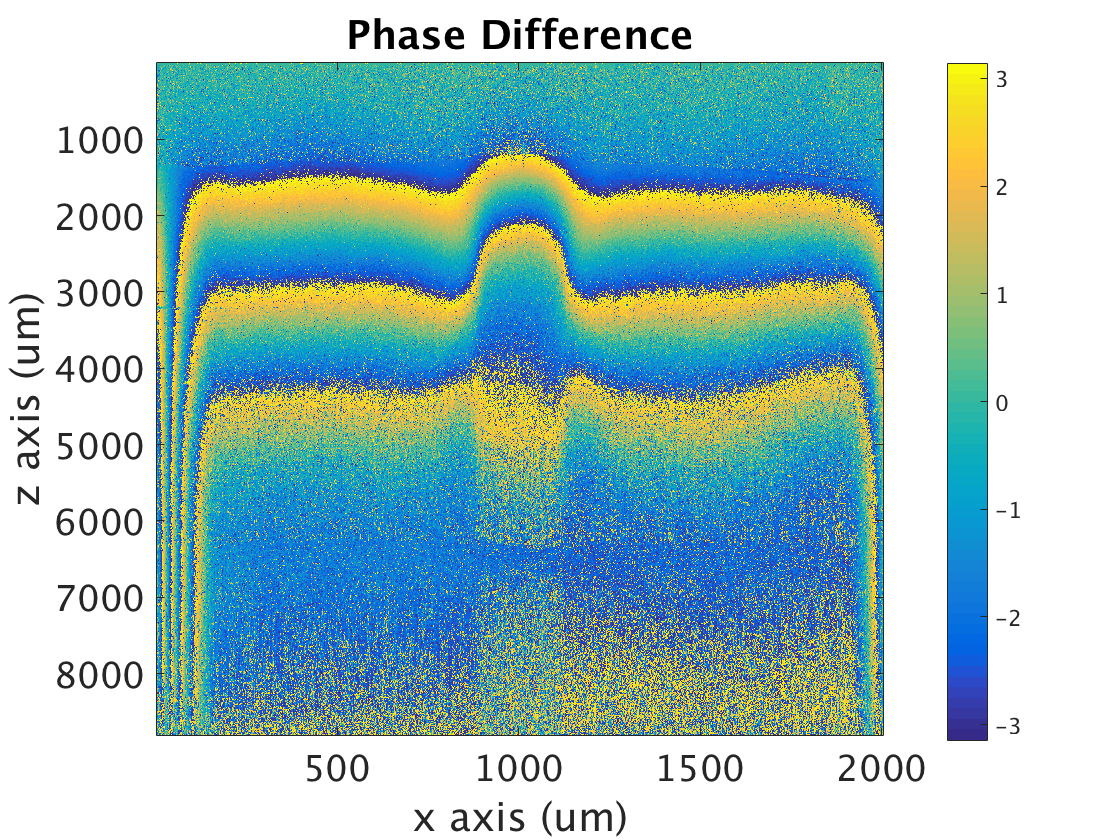
\includegraphics[width=\textwidth]{figures/phase_difference.png}
	\end{subfigure}
	\begin{subfigure}{0.49\textwidth}
		\centering
		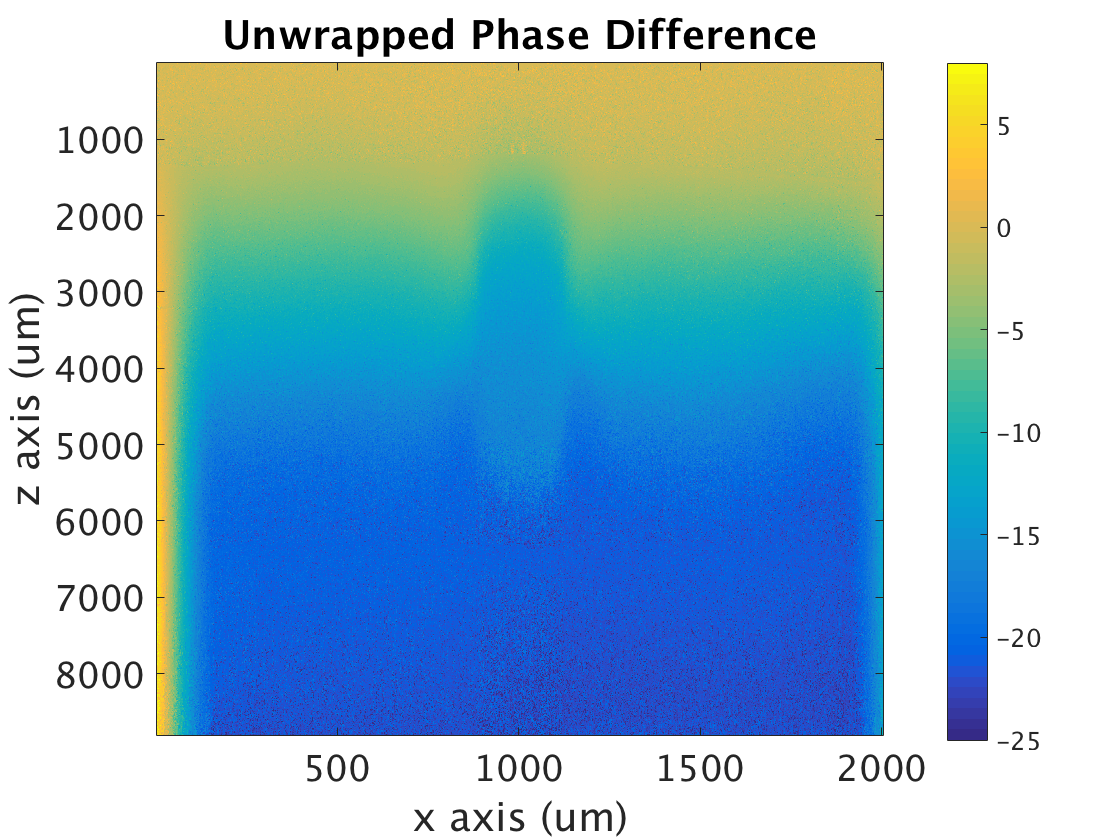
\includegraphics[width=\textwidth]{figures/unwrapped_phase.png}
	\end{subfigure}
	\label{phase_wrapping}
	\caption{Phase unwrapping demonstrated in a phantom scan data set in a) followed by the unwrapped phase difference b) computed using the unwrapping algorithm from \cite{kennedy_optical_2014}.}
\end{figure}


The efficiency of any elastography imaging technique is dependent on its ability to measure the deformation of the tissue in response to the mechanical load accurately. Phase-sensitive displacement measurement in OCE is enabled by Fourier-domain OCT systems, and allows tissue displacements on the order of nanometres to be detected by the system, corresponding to micro-strain sensitivity \cite{kennedy_review_2014}. However phase-sensitive OCE methods bring with them their own problems, one being that te detected phase can only take values in the interval $[0,2\pi]$. This results in wrapping of the phase difference as seen in Figure \ref{phase_wrapping} and if uncorrected, will result in discontinuities in the calculated displacement field.

\subsection{Phase Unwrapping}
To prevent phase wrapping in phase-sensitive displacement measurements, the difference in displacement between loaded and unloaded scans must be limited to approximately $0.3-0.46\mu m$ \cite{kennedy_optical_2014}. However in most instances, the amount of compression applied in OCE in order to produce images with sufficient contrast results in displacements large enough to induce phase wrapping in the signal. Therefore the issue of phase wrapping must be tackled in some way. Three different techniques of phase unwrapping are discussed in this project. The first technique is to implement a phase unwrapping algorithm that loops through the data set and detects wrapping events. This algorithm is more completely described elsewhere \cite{kennedy_optical_2014} however at a high level, it works under the assumption that displacements induced at a given depth is uniform over a local region, and performs first axial then lateral unwrapping. The phase difference is assumed to be unwrapped over an initial depth segment, for which a mean phase value is calculated. From here, each subsequent voxel in depth has an integer number of $2\pi$ subtracted from it based on minimising the difference between its phase value and the preceding mean value, in order to axially unwrap. The lateral unwrapping is performed in a similar way, except by minimizing the difference between the phase at a given voxel with the averaged phase of its lateral neighbours. It has been demonstrated that the algorithm can remove up to 5 wrapping discontinuities \cite{kennedy_optical_2014} before artifacts become prominent.
The benefit of the phase unwrapping algorithm is that it is capable of returning the reconstructed displacement field of the entire B-scan. 

\begin{figure}[b]
	\centering
	\begin{subfigure}{0.25\textwidth}
		\centering
		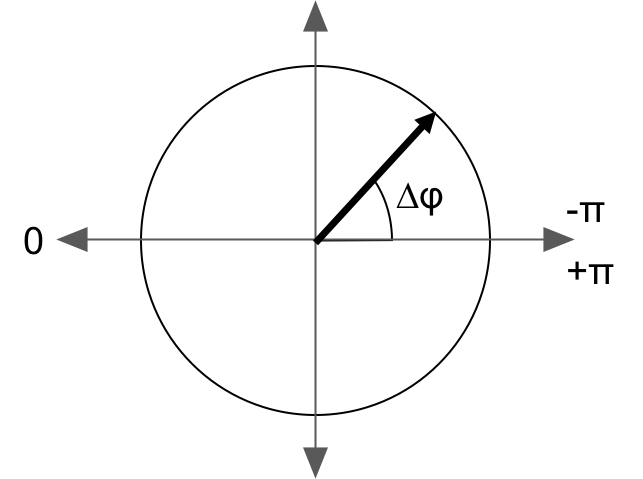
\includegraphics[width=\textwidth]{figures/cplx_phasedif_phasor.png}
	\end{subfigure}
	\quad
	\begin{subfigure}{0.25\textwidth}
		\centering
		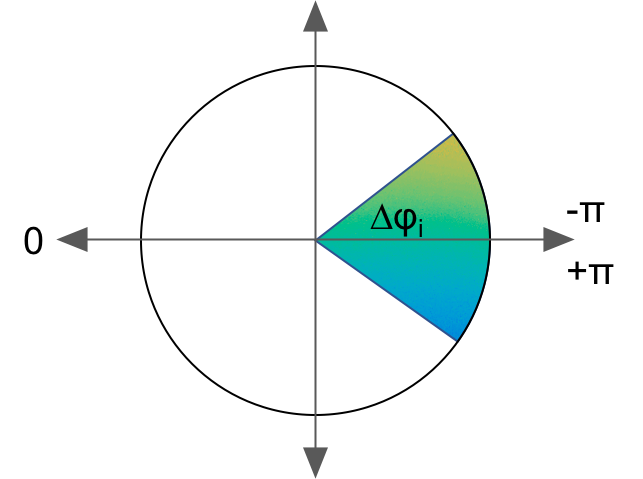
\includegraphics[width=\textwidth]{figures/cplx_phasedif_segment.png}
	\end{subfigure}
	\quad
	\begin{subfigure}{0.25\textwidth}
		\centering
		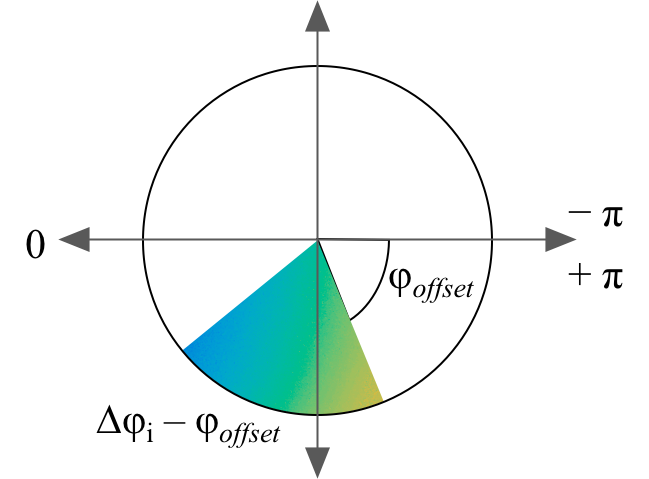
\includegraphics[width=\textwidth]{figures/cplx_segment_shifted.png}
	\end{subfigure}
	\label{phase_offset}
	\caption{The complex phase difference signal using phasor representation in a) as a single data point, b) as a fit window of phase difference data points wrapped around the $\pi/\pi$ discontinuity, and c) those data points shifted to an unwrapped region, based on application of a phase offset \cite{zaitsev_hybrid_2016}.}
\end{figure}

\subsection{Phase Offset Correction}
An alternative approach to the phase wrapping issue was investigated by Zaitsev et.al. \cite{zaitsev_hybrid_2016}, based on the fact that the underlying displacement field does not have to be extracted for the entire scan to produce a strain elastogram, but alternatively only the gradient within the fitting window must be maintained and extracted. In this case the phase unwrapping algorithm is dropped, and a complex phase offset is subtracted from each fit segment to remove any possible wrapping event by returning it to an unwrapped region, as shown in Figure \ref{phase_offset}. From here the strain is estimated using the unwrapped fit segment. This method obviously falters when there are multiple wrapping discontinuities within a given strain fit window, however this is unlikely given most strain estimation techniques maintain smaller fit windows to increase the resulting axial resolution.
Subtraction of a complex phase offset is a non-linear filter operation, and therefore must be performed on each fit segment separately. For strain estimation filter methods (discussed in Chapter 3) this bottleneck slows down the strain estimation process for methods that use a phase offset to unwrap, however it can be mitigated by methods described in the next section.

\subsection{Alternative Approaches}
A third range of approaches do not tackle the issue of phase unwrapping directly, but rather makes the fit segment so small it is assumed no wrapping can occur between. Using finite difference to calculate the strain, performed on the complex phase, ensures that no wrapping artefacts enter the image, provided that no wrapping events occur between consecutive pixels, which is a valid assumption with the amount of compression used. The down side to this technique is that finite difference and any other technique that uses a very small fit window to mitigate phase unwrapping issues is a noisy differentiation method, and results in significant degradation of image quality when used alone. The following Chapter discusses such strain estimation methods in more detail, separate to the issue of phase unwrapping.
          
\chapter{Review of Strain Estimation Techniques}\label{review}

Imaging strain is one fundamental application of OCE, which produces qualitative images of the stiffness of tissue. The tissue strain is defined as the amount of displacement induced in the tissue by the mechanical loading per spatial region. It is calculated by estimating the spatial derivative of the displacement imaged by the OCE system. 

Most elastography techniques utilise the assumption that tissue is a linearly elastic solid \cite{kennedy_review_2014}, an assumption that is valid for applications of small mechanical loads, and that greatly simplifies elastogram processing. Making this assumption, the displacement can be thought of as linearly related to the depth into the sample. Under small enough compressions this assumption is valid. 

To be able to compare between imaging techniques, the resolution of different strain estimation fits must be derived. This resolution can be thought of as the full-width at half maximum of the impulse response of the filter - that is, the FWHM of the output when the input signal is a delta function in the case of a smoothing filter, or a step function for the differentiation filters. This resolution offers a comparative measure of the extent to which the filtering process has blurred objects in the image together. 

\section{Least Squares Approaches}\label{least_squares}
Least squares approach aim to fit a straight line to the phase data by minimising the squared error between the fitted and actual values. The strain value is then taken to be the gradient of this line. The ordinary least squares estimate for the strain value within a fit window of size $m$ is given in \cite{kennedy_strain_2012} as:

\begin{equation}
	\label{ols_strain}
	\epsilon_z = \sum\limits_{j=1}^{j=i+m-1} \bigg(\frac{\kappa_0 (z_j-z_{i-1})-\kappa_1}{\kappa_0 \kappa_2 - \kappa_1^2} \bigg) u_j
\end{equation}

Where $u_j$ is the displacement at the point, and the simplifying constants $\kappa_x$ are defined as:

\begin{equation}
	\label{ols_k}
	\kappa_x = \sum \limits_{j=1}^{i+m-1} (z_j - z_{i-1})^x \text{   for   } x = 0,1,2
\end{equation}

Depending on the size of the fit window, there is a likelihood of a wrapping event to have occurred, and therefore there is a need to unwrap the phase (displacement) data prior to performing a least squares estimate. 

The ordinary least squares estimate above is a linear operation, however can be extended to use weight the contribution of each displacement point based on the quality of its signal. The weighted least squares strain estimate utilises the OCT signal attached to each phase difference value to provide an estimate of the standard deviation of each point. The variance of the measured phase difference is equal to the inverse of the SNR of the OCT intensity, $SNR_{OCT}$. Therefore a $\Delta \phi_i$ measurement that has a high $SNR_{OCT}$ has a low variance, and should be assigned more significance in estimating a linear displacement fit. Therefore the weights associated with the weighted least squares estimate is the inverse variance of the phase difference values:

\begin{equation}
	\label{wls_w}
	w_i = \frac{1}{\sigma_{u_j}^2} = SNR_{OCT_j}
\end{equation}

Using these weights, the strain estimate using weighted least squares is given as in \cite{kennedy_strain_2012} by \autoref{wls_strain}:

\begin{equation}
	\label{wls_strain}
	\epsilon_i = \sum \limits_{j=1}^{i+m-1} \frac{\kappa'_0 w_j (z_j - z_{i-1}) u_j - \kappa'_1 w_	j u_j}{\kappa'_0 \kappa'_2 - (\kappa'_1)^2}
\end{equation}

Where in this instance, the $\kappa'_x$ constants are given by:

\begin{equation}
	\label{wls_k}
	\kappa'_x = \sum \limits_{j=1}^{i+m-1} w_j (z_j - z_{i-1})^x \text{   for   } x=0,1,2
\end{equation}

The weighted least squares strain estimate has been shown to improve the strain sensitivity \cite{kennedy_strain_2012} however at the expense of requiring the calculation of the weightings, and the non-linearity of the operation, the consequences of which are discussed in the next section.

\section{Savitzky-Golay Filtering}\label{sg_filter}
One benefit of the ordinary least squares approach is that it can be implemented as a filter, since it is a linear operation. The Savitzky-Golay filter \cite{savitzky_smoothing_1964} can be applied to data to smooth it to a linear fit, equivalent to performing a least squares estimate. This filter can be applied to an entire data set by convolving the data and filter together, or a multiplying them in the Fourier domain. Similarly to how the estimate above for ordinary least squares is derived using the normal equation for least squares minimization (see \autoref{normal_equations}), the Savitzky-Golay filter is derived by assuming the data is centred around zero and scaled in integer steps, and calculating the filter coefficients for these points for the given fitting model (in this case, linear), and then generalising them to all fit windows. A more detailed derivation can be found in \cite{savitzky_smoothing_1964}. The Savitzky-Golay smoothing filter based on the least squares approximation can be generalised to a Savitzky-Golay differentiation filter by evaluating the gradient, rather than the value, at each point. There is an analytical solution for the Savitzky-Golay first order differentiation filter for a linear least squares model given in \autoref{sg_coeff} \cite{madden_comments_1978}.

\begin{equation}
	\label{sg_coeff}
	C_i = \frac{12 i}{m(m^2-1)}
\end{equation}

Therefore not only can the filter be applied much faster than a sequential looping over the fit windows and performing the ordinary least squares estimate above, it can be created very quickly as well. However, the weighting information can no longer be utilised in the convolution process. Another aspect to note, is that the Savitzky-Golay filter can only be applied on the unwrapped phase difference - it cannot correct for wrapping events. 

The resolution of the Savitzky-Golay filter can be derived by analysing it's response to an impulse. It can be seen that the impulse response of the filter is quadratic in form, and the FWHM can be solved for, giving the value in \autoref{sg_fwhm}:

\begin{equation}
	\label{sg_fwhm}
	\text{FWHM}_{SG} = \frac{m}{\sqrt{2}}
\end{equation}

\section{Smoothing Filters}
In most biological signal processing, high frequency noise is a significant degrading factor, one that is amplified in applications such as elastograpy where derivatives are estimated to produce the signal \cite{usui_digital_1982}. As a result, low-pass differentiation filters are ideal signal processing techniques. The Savitzky-Golay filter acts as a low-pass differentiation filter \cite{luo_axial_2004}, as does a sequential application of weighted least squares. However the simple finite difference strain estimation described in \autoref{fd} makes no effort to smooth out high frequency noise. It makes sense to combine a low-pass smoothing filter with the finite difference derivative estimation in order to do this. Since linear filter operations are commutative, the filter convolution operation can be done to the phase difference or to the finite difference strain estimate. This smoothing filter could be implemented as a simple moving average, however with the goal of minimising the contribution of high frequency noise, it makes sense to take a Gaussian smoothing filter, the discretised version of which is seen in \autoref{gauss_1d} for a 1D filter, and \autoref{gauss_2d} for the 2D filter.

\begin{equation}
	\label{gauss_1d}
	G^{1D}_i = \frac{1}{\sqrt{2\pi} \sigma} \exp{\bigg(\frac{-(i_0-i)^2}{2 \sigma^2}\bigg)}
\end{equation}

\begin{equation}
	\label{gauss_2d}
	G^{2D}_{ij} = \frac{1}{2\pi \sigma_i \sigma_j } \exp{ 
	\bigg( - \frac{(i_0 - i)^2}{2 \sigma_i^2} - \frac{(j_0 - j)^2}{2 \sigma_j^2} \bigg)}
\end{equation}

Using a Gaussian smoothing filter in addition to finite difference removes high frequency noise, where the resolution of this smoothing filter is defined as the FWHM of the Gaussian filter used, dependent on the $\sigma$ value as shown in \autoref{gauss_fwhm}.

\begin{equation}
	\label{gauss_fwhm}
	\text{FWHM}_{Gaussian} = 2 \sqrt{2 \log{2}} \sigma
\end{equation}

\section{Finite Difference}\label{fd}
The simplest approximation to a derivative is to calculate the finite difference between two consecutive displacement measurements. That is, dividing the change in displacement by the change in depth, as per \autoref{fd_strain}.

\begin{equation}
	\label{fd_strain}
	\epsilon_z = \frac{\Delta u_z}{\Delta z}
\end{equation}

An issue with finite difference approaches is that they tend to amplify high frequency noise in the phase values. However one of its benefits is the simplicity of implementation, and therefore the speed up it offers. In addition, by using consecutive pixels to perform the differentiation, there is little chance of a phase wrapping event to have occurred, and therefore finite difference can be performed on the complex phase data without prior unwrapping.

Since there is no smoothing operation implemented in finite difference, it is assumed that it has no effect on the resolution of the image. Therefore there is no assumed a negligible fit resolution contribution using the finite difference strain estimation, and the fit resolution is instead defined by smoothing operations that are implemented alongside it.

\section{Strain Estimation Assessment Criteria}\label{criteria}

\subsection{Sensitivity}
The strain sensitivity is defined as the minimum detectable strain in the elastogram \cite{kennedy_strain_2012}, a quantity that gives insight into how well the OCE imaging system and signal processing is capable of reproducing the physical displacement and strain in the imaged sample. If the strain sensitivity is too large, then it is not possible to detect differences between stiff and soft objects (such as stroma and tumour) without having a much larger compressive force, which invalids many assumptions previously made (such as the linear elasticity of tissue, and uniaxial compression). Therefore it is important to use the strain sensitivity as a metric of image quality. 

The strain sensitivity is defined as the standard deviation of the strain values within a region of uniform elasticity \cite{varghese_theoretical_1997}, such as can be artificially created using a phantom. The ideal characteristics of the region include absence of artefacts, including those that occur near the sample surface reflection, and at a depth shallow enough to minimise the attenuation of the OCT signal and decorrelation noise. Such a region is shown in \autoref{sensitivity_region} for a silicon phantom with a stiff inclusion. 

\subsection{Image Resolution}
The image resolution can be thought of as the ability to distinguish between two objects in the resulting strain elastogram. Traditionally, this has been examined in terms of the impulse response of an optical system, more directly as the FWHM of this impulse response \cite{reynolds_resolution_1989}. However we typically don't have access to the impulse response of the combined strain estimation filter and optical system response, therefore another method of quantifying the image resolution is used based on a previous Masters project \cite{hepburn_improving_2017}.

\begin{figure}[t]
	\centering
	\begin{subfigure}{0.49\textwidth}
		\centering
		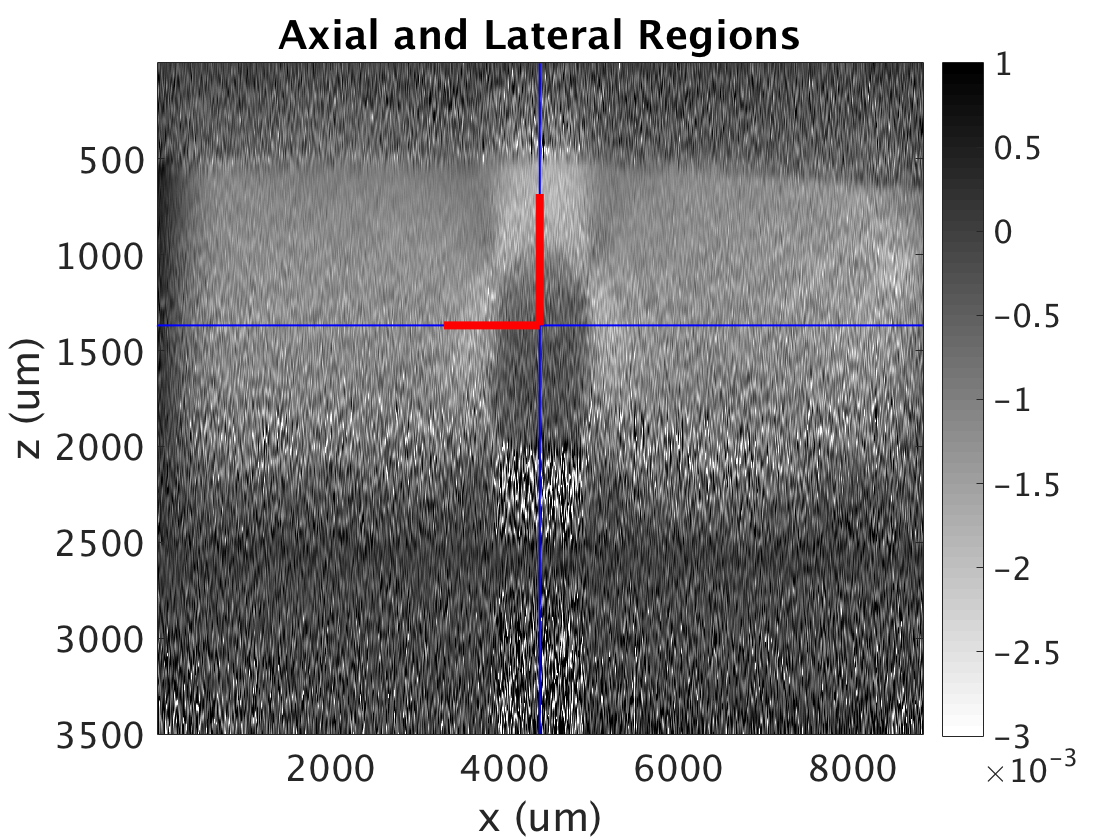
\includegraphics[width=\textwidth]{figures/image_res_regions.png}
	\end{subfigure}
	\begin{subfigure}{0.49\textwidth}
		\centering
		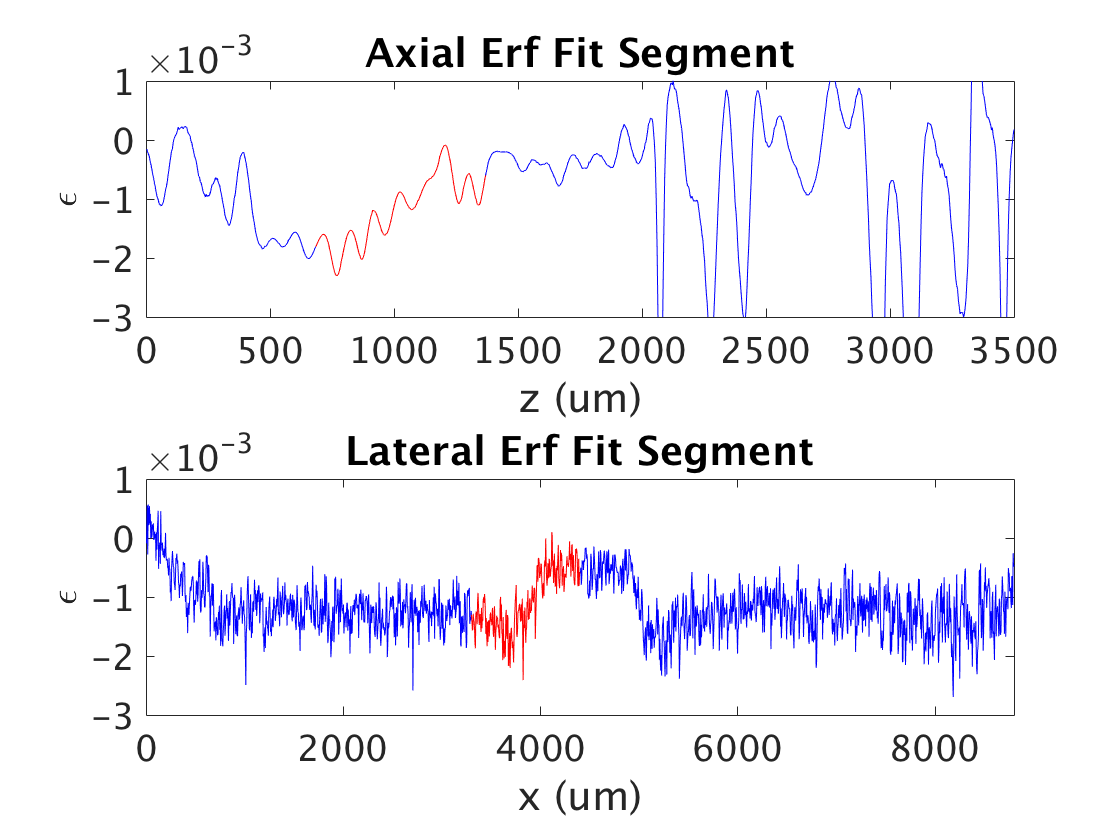
\includegraphics[width=\textwidth]{figures/lateral_axial_segments.png}
	\end{subfigure}
	\caption{The segments used to calculate the image resolution for both axial and lateral directions, shown imposed on the strain elastogram in a) where the blue corresponds to the scan taken, and the red the region the error function is fitted over. Part b) shows the plots of these scans and segments, with the axial above, and lateral below.}
	\label{axial_lateral_regions}	
\end{figure}

The image resolution is thought of as the 'speed' of transition from one uniform strain region to another, as measurable in a phantom sample which has clearly defined regions of different stiffness. This transition can be seen in both the axial and lateral directions, as shown in \autoref{axial_lateral_regions}.

\begin{figure}[t]
	\centering
	\begin{subfigure}{0.49\textwidth}
		\centering
		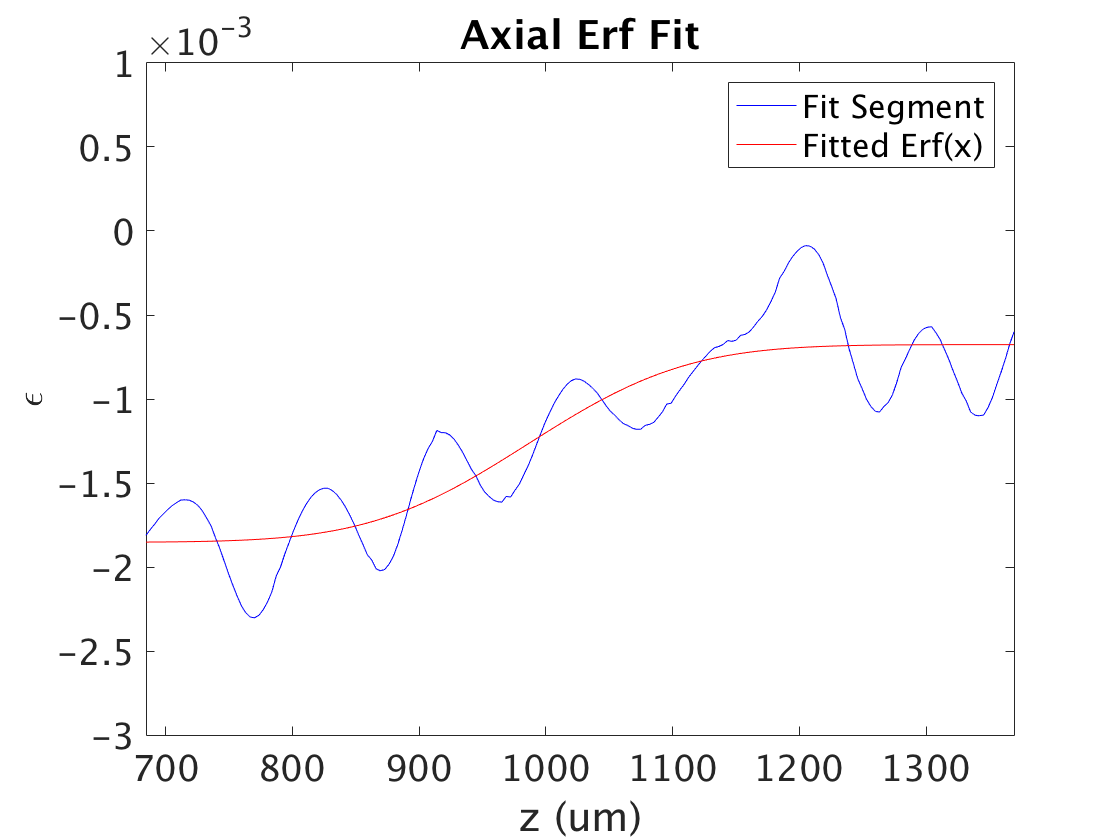
\includegraphics[width=\textwidth]{figures/axial_erf_fit.png}
	\end{subfigure}
	\begin{subfigure}{0.49\textwidth}
		\centering
		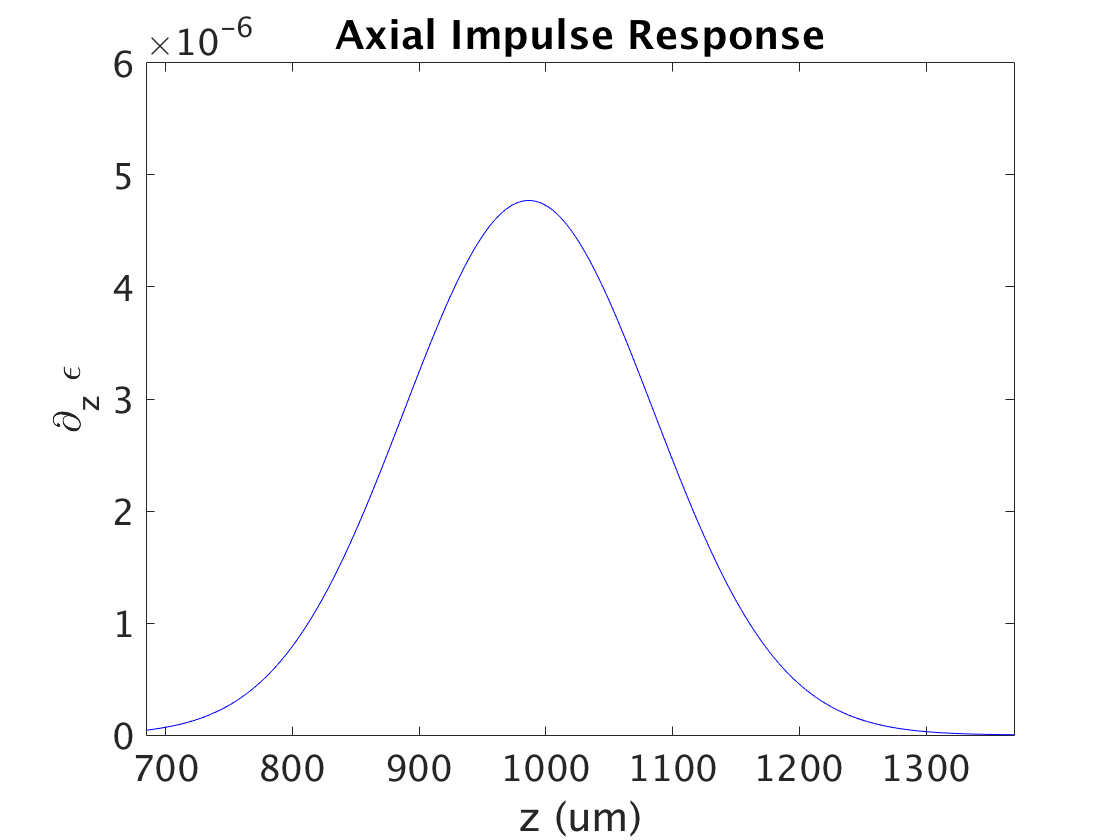
\includegraphics[width=\textwidth]{figures/axial_impulse_response.png}
	\end{subfigure}
	\\
	\begin{subfigure}{0.49\textwidth}
		\centering
		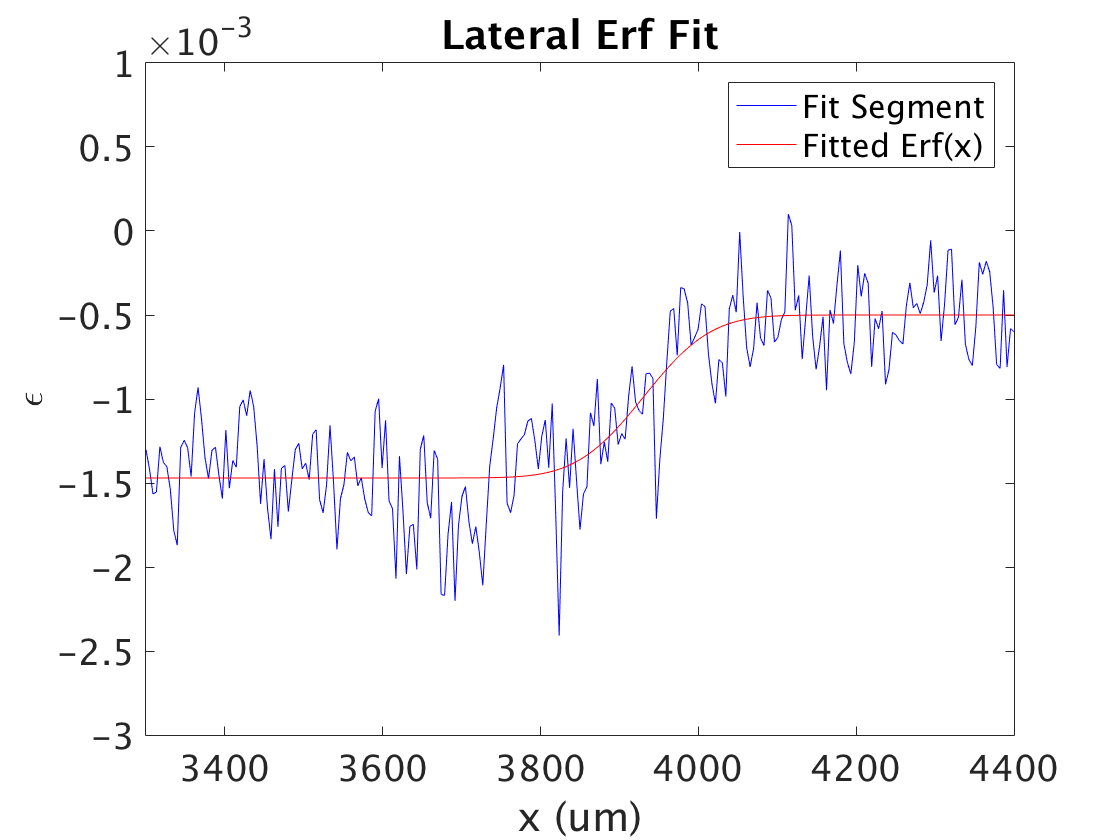
\includegraphics[width=\textwidth]{figures/lateral_erf_fit.png}
	\end{subfigure}
	\begin{subfigure}{0.49\textwidth}
		\centering
		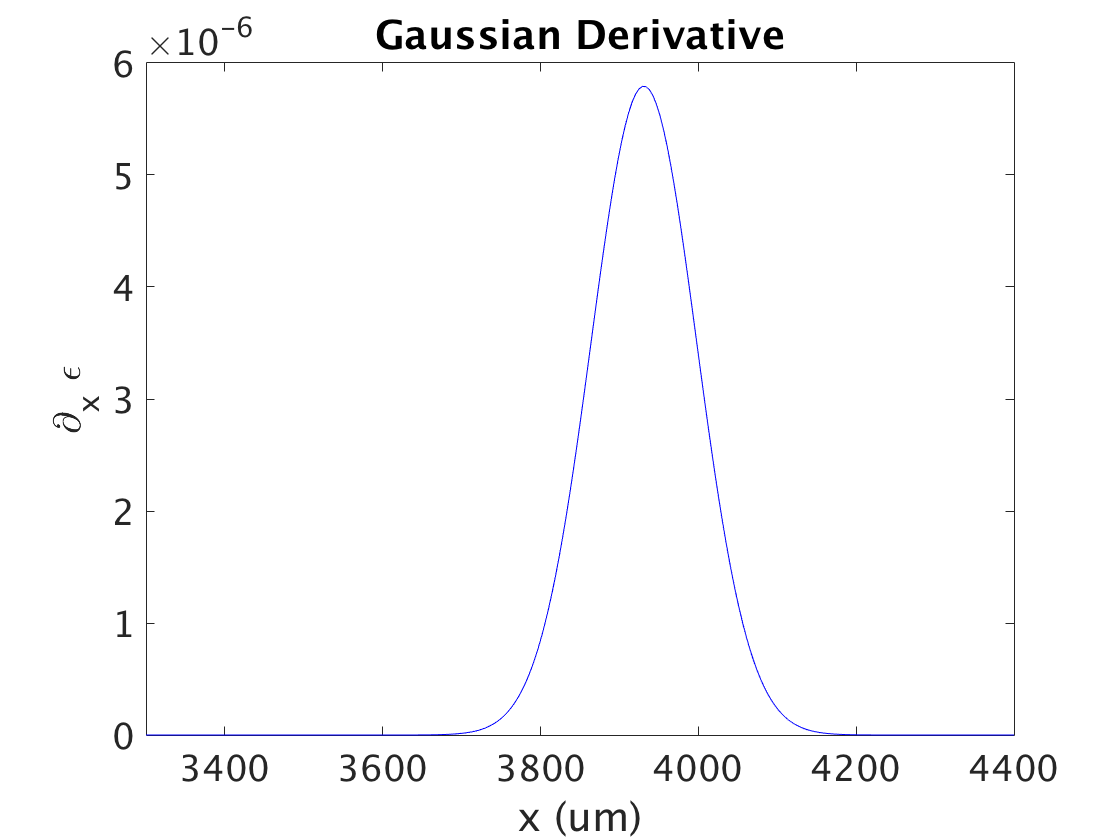
\includegraphics[width=\textwidth]{figures/lateral_impulse_response.png}
	\end{subfigure}
	\caption{The left images show the segment over the axial and lateral boundaries respectively with the overlaid error function fit. The right images show the impulse response, which is the derivative of the error function, for the fit, of which the FWHM is the image resolution.}
	\label{error_fit_example}	
\end{figure}

The transition across a feature boundary in the strain elastogram can be approximated by an error function, as given in \autoref{erf_normal}, and visualised in \autoref{error_fit_example}. 

\begin{equation}
	\text{erf}(x)=\frac{1}{\sqrt{\pi}} \int_{-x}^{x} \text{e}^{-t^2}
	\label{erf_normal}
\end{equation}

The standard error function above can be translated and scaled (see \autoref{erf_scaled}) to allow fitting to the strain values over the boundary, and also to allow for the introduction of the parameter $a$ that governs the rise time of the error function. When this scaled error function is fitted to the strain data across the boundary, the $a$ parameter is the most significant and is used to calculate an image resolution.

\begin{equation}
	n \: \text{erf}(\:a(x-b)\:) + c = \frac{n}{\sqrt{\pi}} \int_{-(x-b)}^{(x-b)} \text{e}^{-a t^2} + c
	\label{erf_scaled}
\end{equation}

Once this analytical model is derived from the strain data, the derivative of the fitted error function provides the impulse response of the system, and it is the FWHM of this derivative that provides the image resolution \cite{hepburn_improving_2017}. For the scaled error function, the derivative is a similarly scaled Gaussian function, given in \autoref{gaussian_derivative}.

\begin{equation}
	G(x) = \frac{2\:a\:n}{\sqrt{\pi}} \text{e}^{-a^2 (x-b)^2}
	\label{gaussian_derivative}
\end{equation}

The FWHM of this Gaussian is given in \autoref{image_res_fwhm} and provides the image resolution in the direction specified (axial or lateral, as in \autoref{axial_lateral_regions}).

\begin{equation}
	\text{FWHM}_{IR} = \frac{2 \sqrt{\text{ln}(2)}}{a}
	\label{image_res_fwhm}
\end{equation}

\subsection{Processing Speed}
The processing speed of the strain estimation technique is not a standard metric for assessing the strain elastogram quality, but keeping in mind the motivation for this project it is of utmost importance.
The processing speed of the different strain estimation algorithms was assessed using both the processing of a single B-scan, and for a complete 3D volume. In addition, differences in algorithm complexity are pointed out between the methods, as well as the ease with which they can be parallelised, and the likelihood of a speed up made possible by parallelising the processing.



         
\chapter{Results}\label{results}


\section{Data Acquisition}\label{data}

\begin{figure}
	\centering
	\begin{subfigure}{0.47\textwidth}
		\centering
		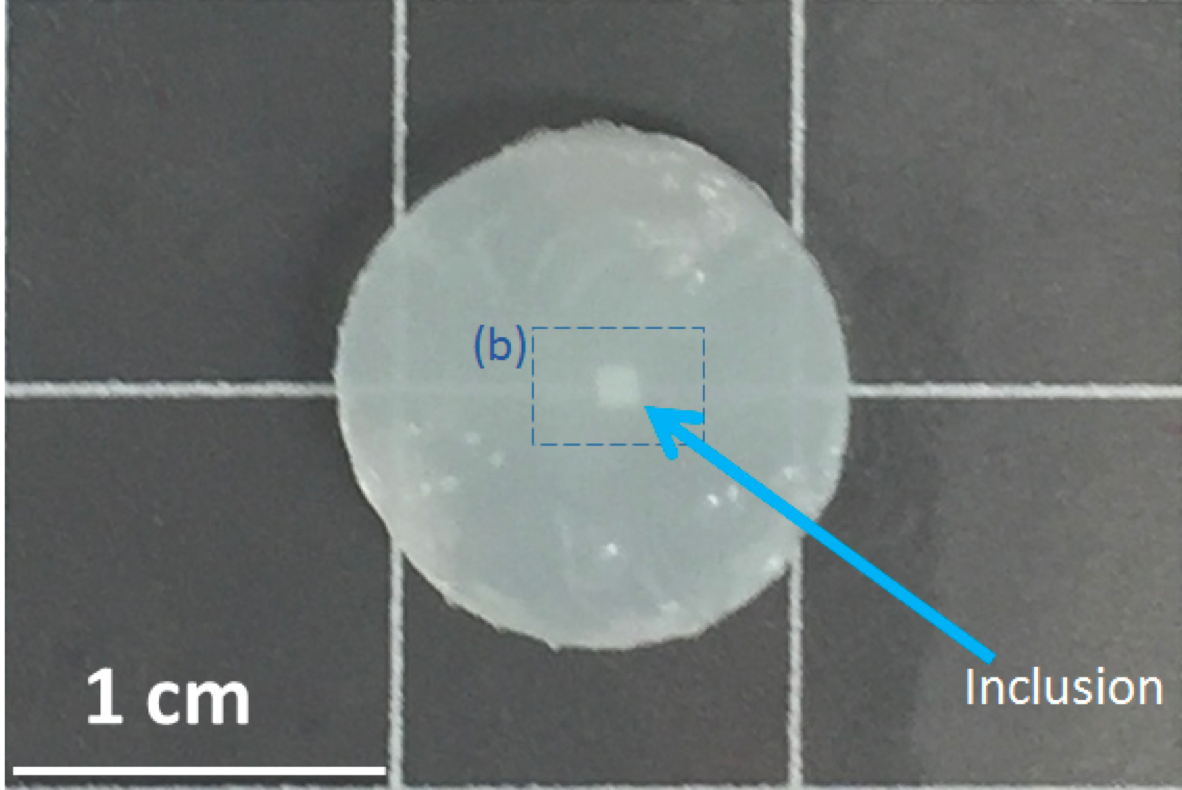
\includegraphics[width=\textwidth]{figures/phantom.png}
	\end{subfigure}
	\quad
	\begin{subfigure}{0.49\textwidth}
		\centering
		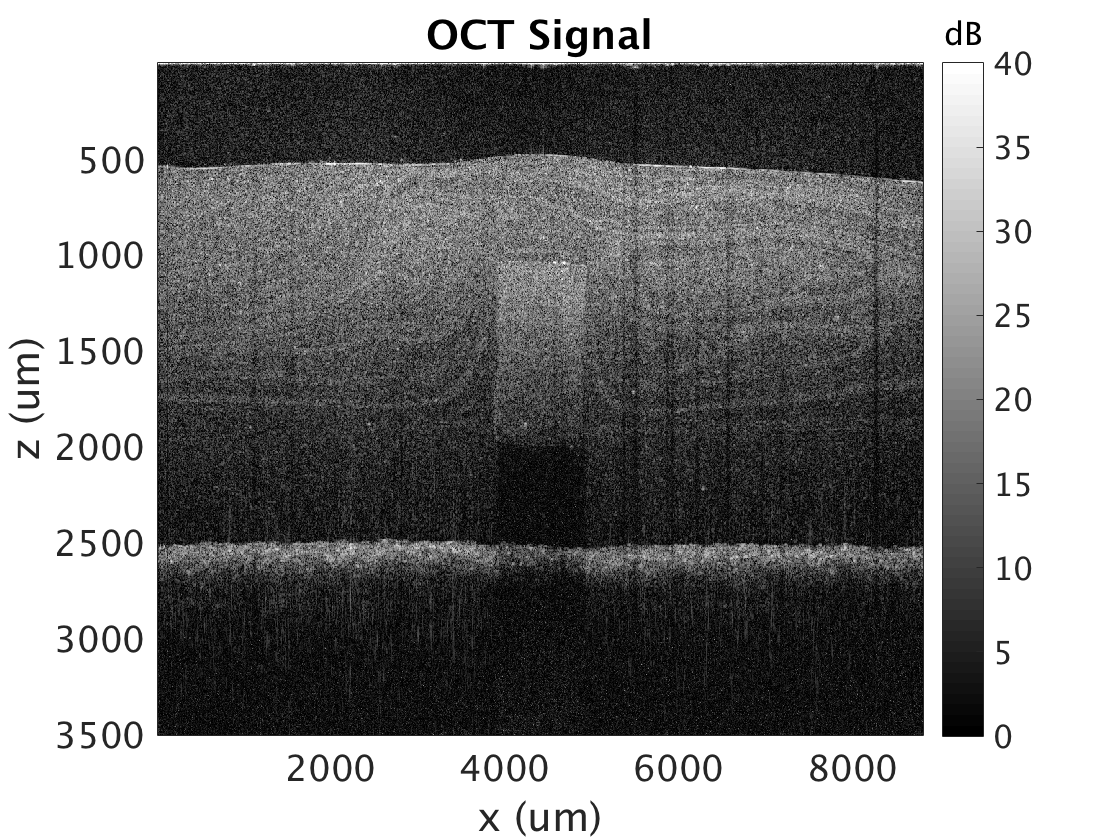
\includegraphics[width=\textwidth]{figures/oct.png}
	\end{subfigure}	
	\caption{The silicone phantom used to investigate strain estimation techniques a) photographed and b) imaged by the OCT system.}
	\label{oct_image}	
\end{figure}

To better quantify the image quality, an idealised silicone sample was imaged, to approximate breast tissue, and the strain estimated. This phantom consisted of a bulk, softer silicone material (with a Young's modulus of 6.4kPa) within which was a stiff, rectangular inclusion (Young's modulus of 100kPa) \cite{hepburn_improving_2017}, to which optical scatterers were added to enhance the OCT signal. The phantom was created by a previous Master's student, and was imaged using a desktop OCE system, with a system wavelength of $1300nm$. The imaged area, shown in \autoref{oct_image}, was divided into 2000 A-scans per each B-scan, over a length in x of $4.4\mu m$), and a total of 6817 B-scans were acquired, over the same length in y.

The complex OCT C-scan was initially processed from the raw spectral data produced by the Fourier-domain OCT system, to produce the complex OCT signal values, with associated optical amplitudes and random phase. From here, as described briefly in \autoref{compression_oce}, the difference in phase is calculated between loaded and unloaded B-scans, and averaged over 100 B-scans. The strain estimation algorithms described following utilise this calculated averaged phase difference as the beginning step of the processing pipeline, and assume that the phase difference data is already loaded into memory.

\section{Strain Estimation Algorithms}\label{algorithms}

A total of six different strain estimation algorithms were implemented and tested, and can be differentiated based on how the phase unwrapping issue is addressed, and the digital differentiation filter used. \autoref{flowchart} demonstrates the decision processes in these strain estimation algorithms that separate the way they get from the complex phase difference delivered by the OCT system and pre-processing, to the final strain elastogram image.
The functions worked by using the complex phase difference C-scan as an input, as well as the specifications for the fit (axial) and lateral resolutions of the system. The fit resolution of the system determined the fit window for the WLS and Savitzky-Golay based strain estimation techniques, and the axial Gaussian $\sigma$ value for the finite difference based techniques. The lateral resolution determined to what extent the strain images were laterally averaged by a Gaussian smoothing filter (for reasons discussed in the later section 4.3). If a lateral resolution of 0 was specified, no lateral smoothing was performed. 

\subsection{WLS with Unwrapped Phase}
The WLS with phase unwrapping algorithm unwraps the phase by reading in the entire volume and saves the unwrapped phase data to file. In a sequential loop over each B-scan, wrapped in a Matlab parfor parallel, the process reads in the complex phase and unwrapped phase for each B-scan. If lateral smoothing has been specified, it smooths the unwrapped phase using unweighted Gaussian smoothing by convoluting the unwrapped phase with the 1D lateral filter. A sequential looping is then performed over each A-scan and all fit segments within the given B-scan, which calculates the WLS estimate of strain using summations and the weights from the complex phase data.

\begin{figure}[th!]
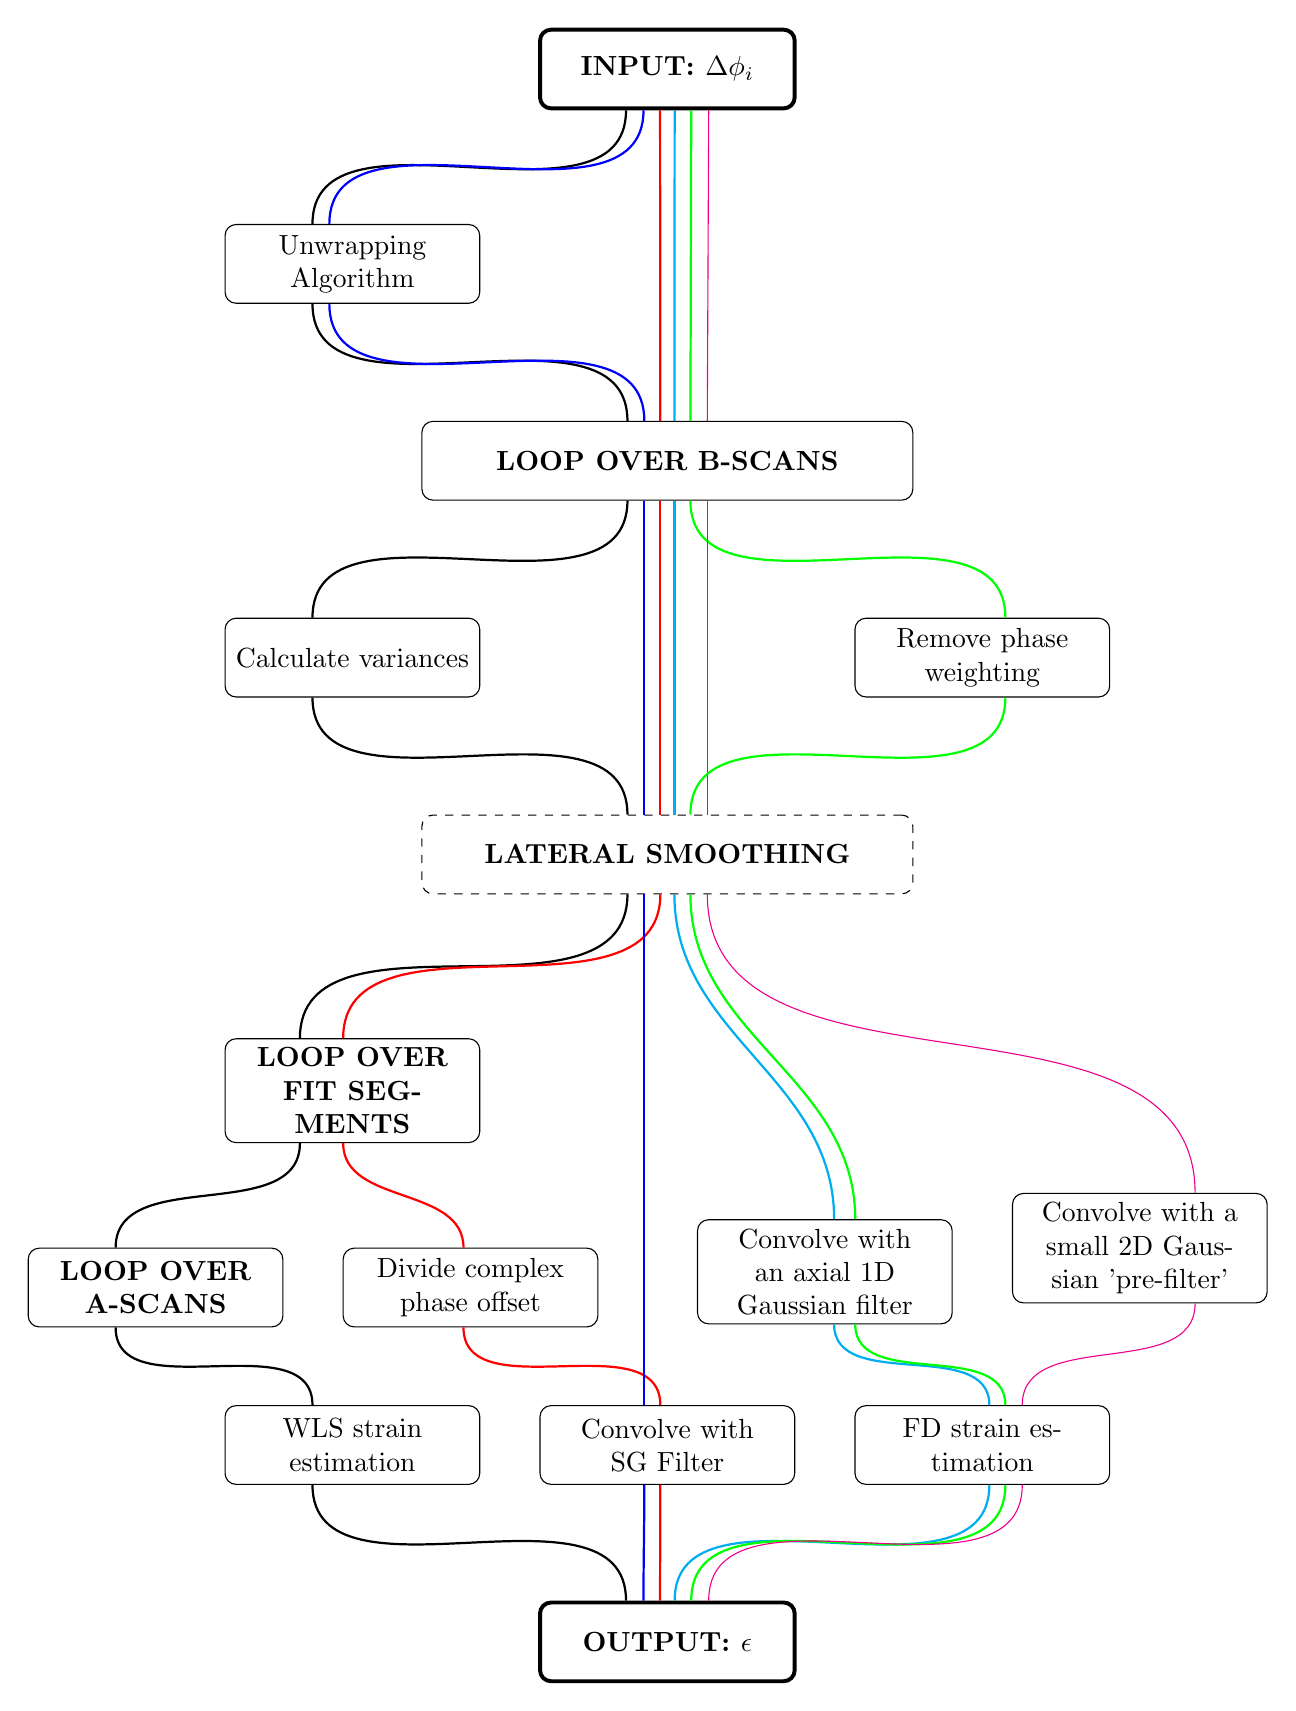
\begin{tikzpicture}[node distance=2cm, remember picture]
	\centering
	\node [anchor=north] at (0,0) (input) [io] {INPUT: $\Delta\phi_i$};
    
    \node (volume_unwrap) at (-4,-3) [basic] {Unwrapping Algorithm};
    \draw [wls] (input.225) edge[out=270,in=90] (volume_unwrap.135);
    \draw [uwsg] (input.240) edge[out=270,in=90] (volume_unwrap.120);
    
    \node (bscan_loop) at (0,-5.5) [main_long] {LOOP OVER B-SCANS};
    \draw [wls] (volume_unwrap.225) edge[out=270,in=90] (bscan_loop.135);
    \draw [uwsg] (volume_unwrap.240) edge[out=270,in=90] (bscan_loop.120);
    \draw [posg] (input.260)--(bscan_loop.100);
    \draw [wfd] (input.280)--(bscan_loop.80);
    \draw [uwfd] (input.300)--(bscan_loop.60);
    \draw [fdsm] (input.315)--(bscan_loop.45);
    
   	\node (variance) at (-4,-8) [basic] {Calculate variances};
    \draw [wls] (bscan_loop.225) edge[out=270,in=90] (variance.135);
    
    \node (unweighted) at (4,-8) [basic] {Remove phase weighting};
    \draw [uwfd] (bscan_loop.300) edge[out=270,in=90] (unweighted.60); 
    
    \node (lateral) at (0,-10.5) [temp] {LATERAL SMOOTHING};
    \draw [uwsg] (bscan_loop.240)--(lateral.120);
    \draw [posg] (bscan_loop.260)--(lateral.100);
    \draw [wfd] (bscan_loop.280)--(lateral.80);
    \draw [fdsm] (bscan_loop.315)--(lateral.45);

	\draw [wls] (variance.225) edge[out=270,in=90] (lateral.135);
    \draw [uwfd] (unweighted.300) edge[out=270,in=90] (lateral.60);
    
    \node (fit_loop) at (-4,-13.5) [main] {LOOP OVER FIT SEGMENTS};
    \draw [wls] (lateral.225) edge[out=270,in=90] (fit_loop.135);
    \draw [posg] (lateral.260) edge[out=270,in=90] (fit_loop.100);
    
    \node (ascan_loop) at (-6.5,-16) [main] {LOOP OVER A-SCANS};
    \draw [wls] (fit_loop.225) edge[out=270,in=90] (ascan_loop.135);
    
    \node (wls_strain) at (-4,-18) [basic] {WLS strain estimation};
    \draw [wls] (ascan_loop.225) edge[out=270,in=90] (wls_strain.135);
    
    \node (phase_offset) at (-2.5,-16) [basic] {Divide complex phase offset};
    \draw [posg] (fit_loop.260) edge[out=270,in=90] (phase_offset.100);
    
    \node (sg_filter) at (0,-18) [basic] {Convolve with SG Filter};
    \draw [posg] (phase_offset.260) edge[out=270,in=90] (sg_filter.100);
    \draw [uwsg] (lateral.240) edge[out=270,in=90] (sg_filter.120);
   
   \node (gauss_filter) at (2,-15.8) [basic] {Convolve with an axial 1D Gaussian filter};
   \draw [wfd] (lateral.280) edge[out=270,in=90] (gauss_filter.80);
   \draw [uwfd] (lateral.300) edge[out=270,in=90] (gauss_filter.60);
   
   \node (pre_filter) at (6,-15.5) [basic] {Convolve with a small 2D Gaussian 'pre-filter'};
   \draw [fdsm] (lateral.315) edge[out=270,in=90] (pre_filter.45);
   
   \node (fd) at (4,-18) [basic] {FD strain estimation};
   \draw [wfd] (gauss_filter.280) edge[out=270,in=90] (fd.80);
   \draw [uwfd] (gauss_filter.300) edge[out=270,in=90] (fd.60);
   \draw [fdsm] (pre_filter.315) edge[out=270,in=90] (fd.45);
   
   \node (output) at (0,-20.5) [io] {OUTPUT: $\epsilon$};
   \draw [wls] (wls_strain.225) edge[out=270,in=90] (output.135);
   \draw [uwsg] (sg_filter.240) edge[out=270,in=90] (output.120);
   \draw [posg] (sg_filter.260) edge[out=270,in=90] (output.100);
   \draw [wfd] (fd.280) edge[out=270,in=90] (output.80);
   \draw [uwfd] (fd.300) edge[out=270,in=90] (output.60);
   \draw [fdsm] (fd.315) edge[out=270,in=90] (output.45);
   
\end{tikzpicture}
\caption{Flowchart of pivotal processes for the six different strain estimation techniques investigated: unwrapping with WLS (black), unwrapping with SG filtering (dark blue), offset phase with SG filtering (red), weighted smoothing with FD (light blue), unweighted smoothing with FD (green), and pre-filtered FD with weighted smoothing.}
\label{flowchart}
\end{figure}

\subsection{SG Filtering on Unwrapped Phase}
This function unwraps the phase by the same process specified above, which requires a read from file of the unwrapped phase for each B-scan. If lateral smoothing required, the unwrapped phase is similarly smoothed via convolution with an unweighted Gaussian smoothing filter. To estimate the strain, this smoothed unwrapped phase data is convolved with the analytically derived Savitzky-Golay filter in a single action of the entire B-scan.

\subsection{SG Filtering on Offset Phase}
In order to correct for phase unwrapping, the function reads in the complex phase for each B-scan (in a parallel Matlab parfor loop) and loops over all fit segments within the B-scan, taking a matrix of values across all A-scans for the given depths. Using Matlab's inbuilt bsxfun operator, an averaged complex phase value for each fit segment is calculated and divided (corresponding to subtraction of the phase) to move the phase values into an unwrapped region. The Savitzky-Golay filter, which was pre-calculated using the analytical solution, is then convolved with the matrix in the axial direction to produce the strain estimation values at that given depth. 

\subsection{FD on Weighted Smoothing of Phase Difference}
The complex weighted phase difference that acts as the function's input is smoothed using an axial Gaussian filter dependent on the fit resolution supplied (and a lateral filter if specified). For strain estimation, finite difference is performed using bsxfun on the complex phase data (in order to prevent the introduction of  wrapping artefacts), by dividing one pixel by the conjugate of the previous pixel in order to subtract the phase values. This estimate of the spatial derivative of the phase difference is then converted into strain values.

\subsection{FD on Unweighted Smoothing of Phase Difference}
This algorithm works almost identically to the one described in the previous section, except that prior to using a Gaussian smoothing filter on the complex phase data, the amplitude is normalised to 1 for all phase difference values, effectively removing the optical weighting that comes from the OCT signal. From here the finite difference is calculated, and from this the strain. 

\subsection{Pre-Filtered Phase Difference with Smoothed FD Strain}
The 'Pre-Filtered' phase difference algorithm was implemented as an effort to remove 'ripples' introduced by high intensity pixels in the finite difference with weighted smoothing described in Section 4.2.4, which will be discussed later in the chapter. Using the weighted complex phase difference data, a small 2D Gaussian filter is applied to smooth out high intensity 'speckle' pixels. This pre-filter is set at $20 \mu m$ resolution, approximately on the order of the speckle size. This action aims to counter the disproportionate influence of high intensity pixels. From here, the strain is estimated using a finite difference, and the resulting strain is smoothed using a 2D Gaussian filter to match the required fit and lateral resolution values. Since the pre-filter contributes to the fit and lateral resolutions, for any given fit resolution $\text{FR}_{total}$ and lateral resolution $\text{LR}_{total}$ supplied to the function as input parameters, the resulting Gaussian smoothing resolutions must take into account the contribution from the pre-filter as in \autoref{prefilter_res_FR} and \autoref{prefilter_res_LR} below.

\begin{equation}
	\text{FR}_{Gauss} = \sqrt{\text{FR}_{total}^2 - \text{FR}_{pre}^2}
    \label{prefilter_res_FR}
\end{equation}

\begin{equation}
    \text{LR}_{Gauss} = \sqrt{\text{LR}_{total}^2 - \text{LR}_{pre}^2}
    \label{prefilter_res_LR}
\end{equation}

In order to maintain consistency between the strain estimation techniques, for the case in which no lateral smoothing is applied for any other algorithms, the pre-filter becomes 1D Gaussian smoothing filter only, so that $\text{LR}_{pre}\rightarrow 0$. 

\section{Phantom Strain Elastogram Results}\label{phantom_results}

\subsection{Qualitative Comparison}

\begin{figure}[b!]
	\centering
    \begin{subfigure}{0.49\textwidth}
    	\centering
        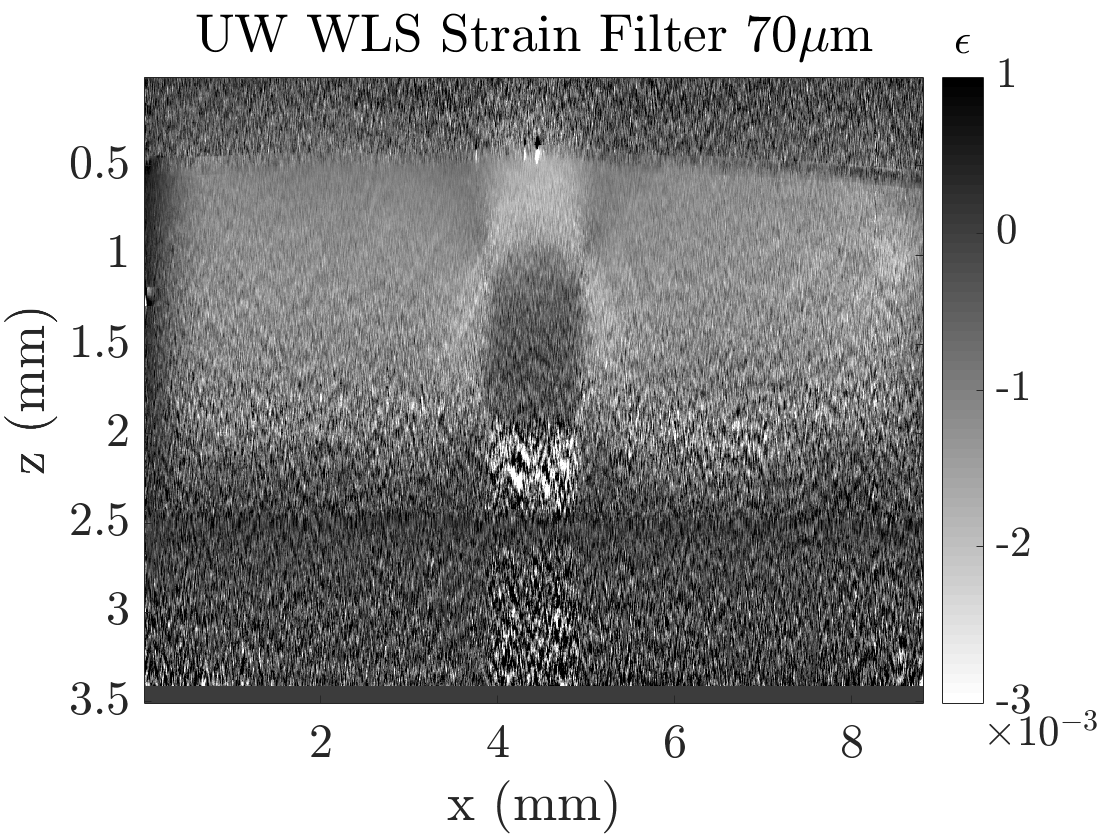
\includegraphics[width=\textwidth]{figures/wls_fr70_lr0.png}
	\end{subfigure}
    \begin{subfigure}{0.49\textwidth}
    	\centering
        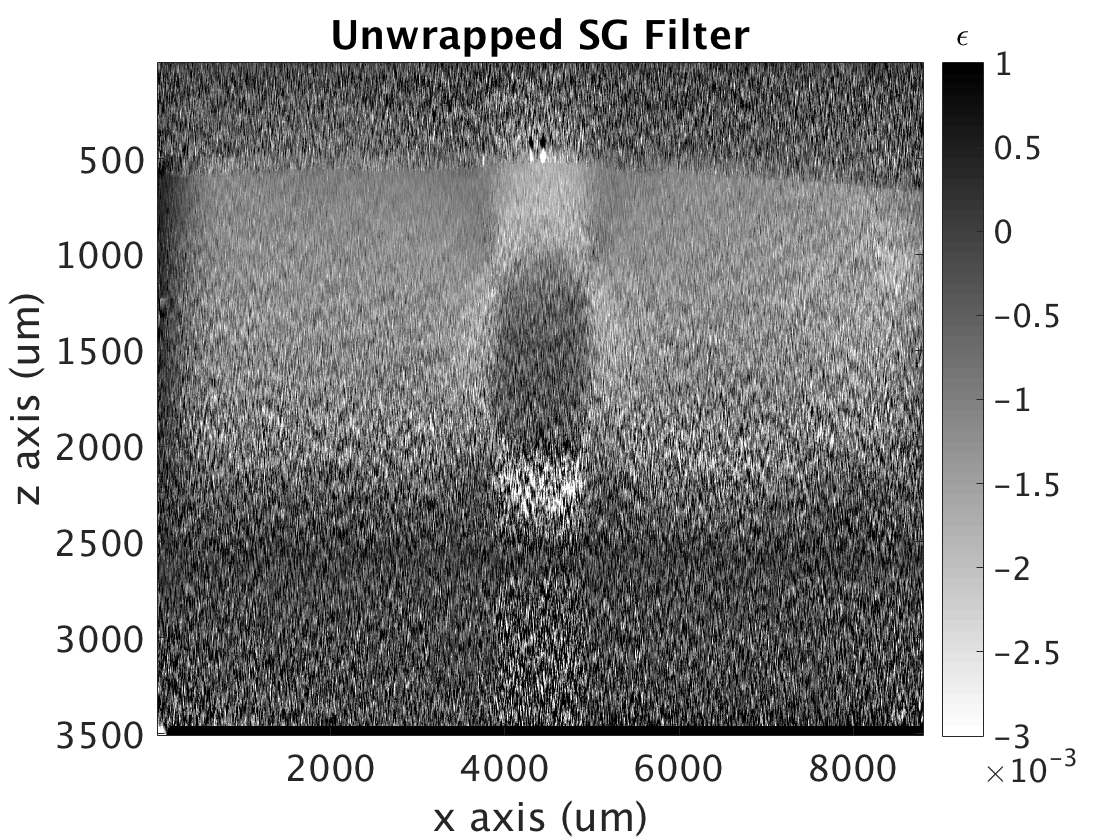
\includegraphics[width=\textwidth]{figures/uwsg_fr70_lr0.png}
	\end{subfigure}
    \\
    \begin{subfigure}{0.49\textwidth}
    	\centering
        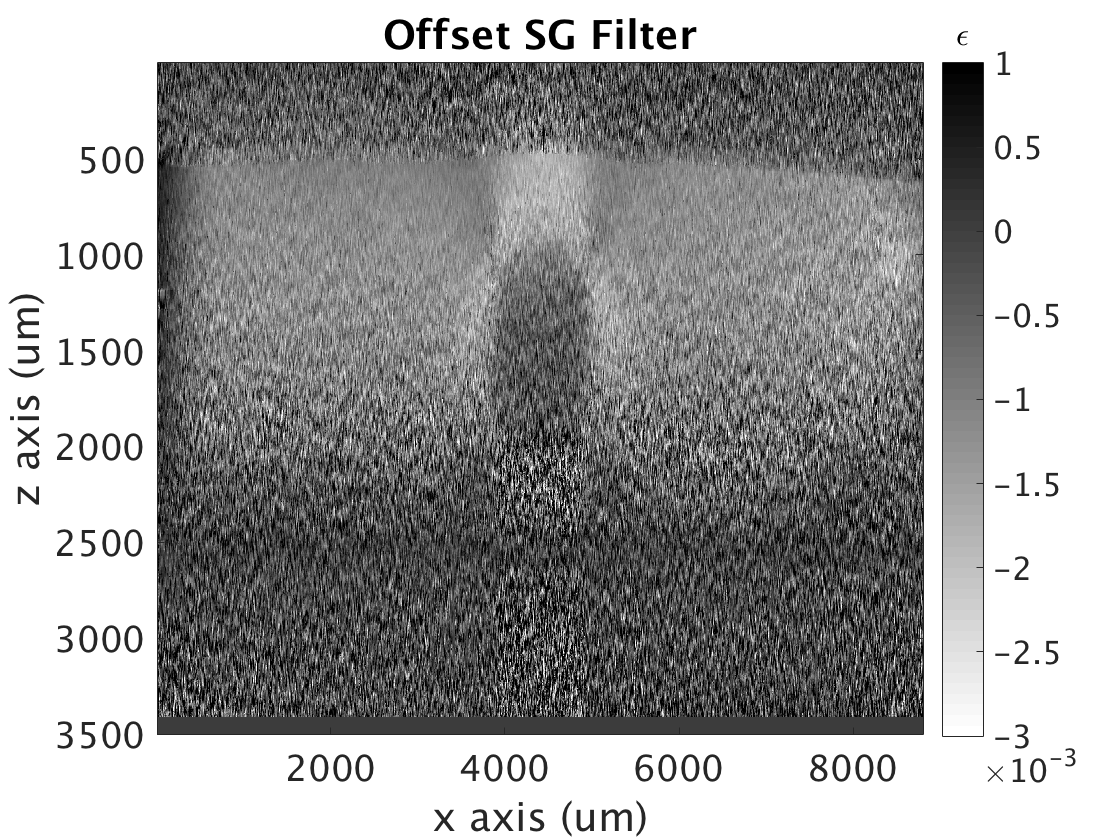
\includegraphics[width=\textwidth]{figures/posg_fr70_lr0.png}
	\end{subfigure}
    \begin{subfigure}{0.49\textwidth}
    	\centering
        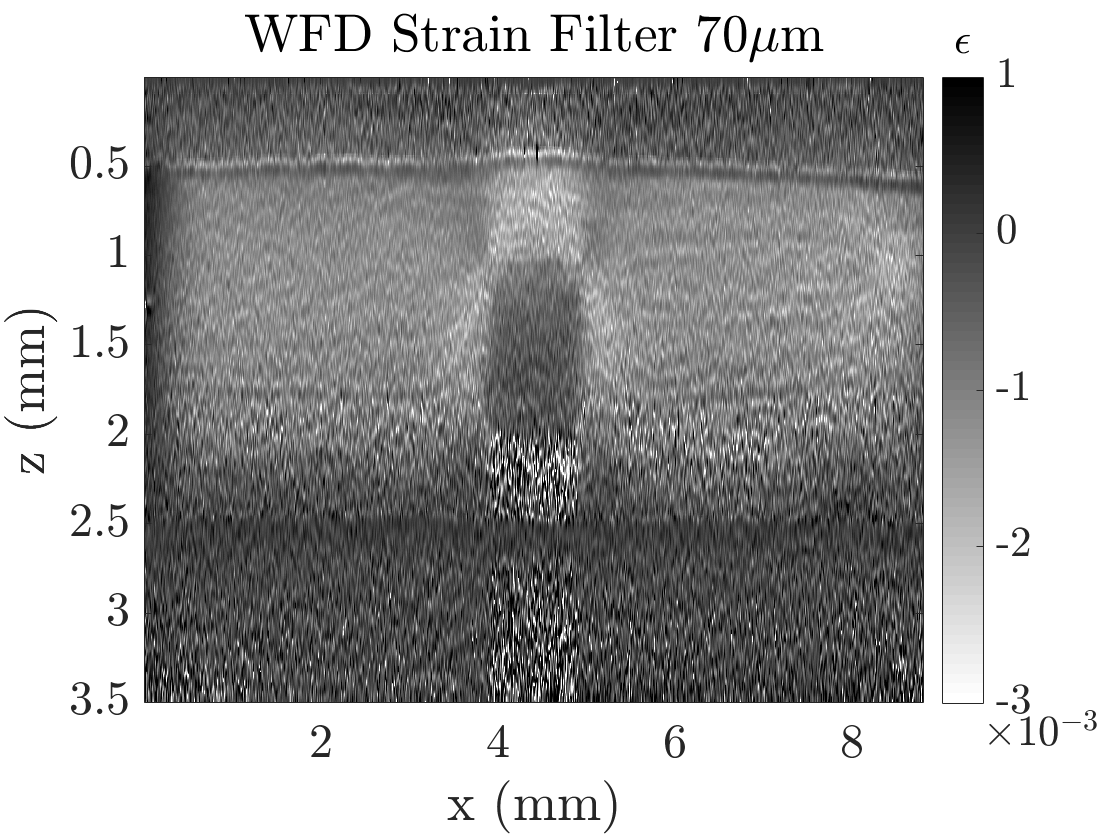
\includegraphics[width=\textwidth]{figures/wfd_fr70_lr0.png}
    \end{subfigure}
    \\
    \begin{subfigure}{0.49\textwidth}
    	\centering
        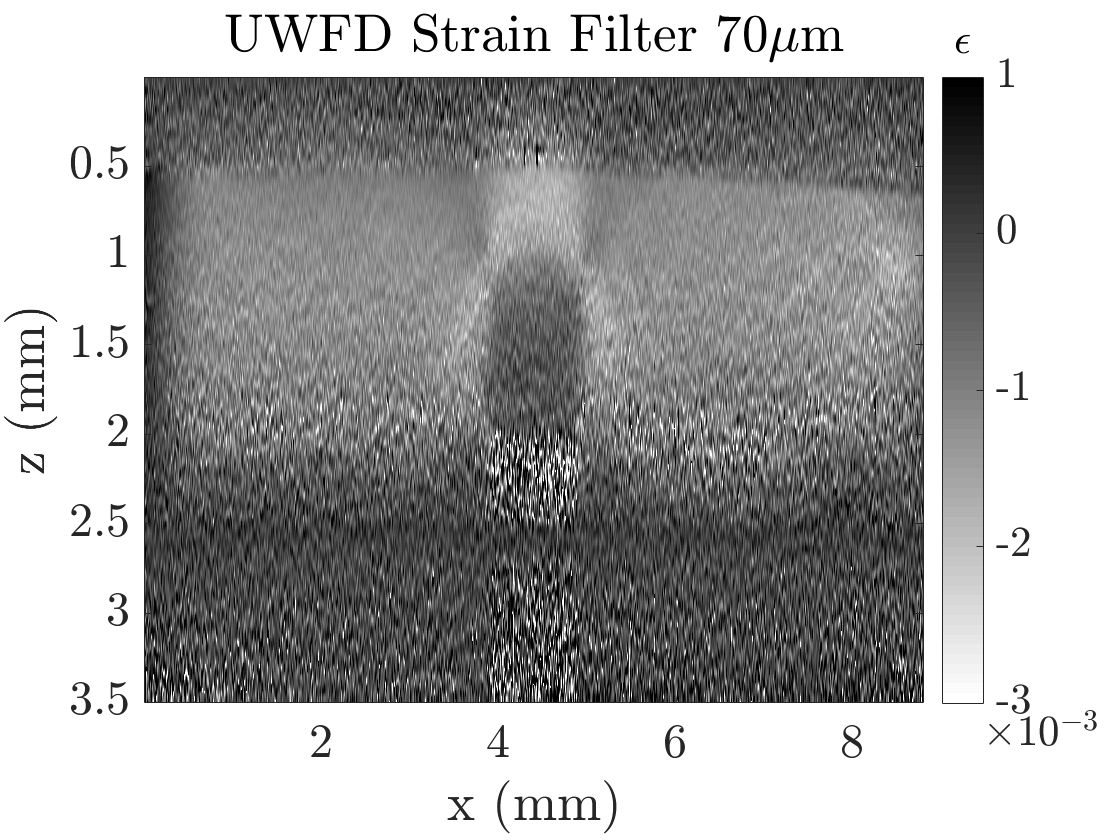
\includegraphics[width=\textwidth]{figures/uwfd_fr70_lr0.png}
	\end{subfigure}
    \begin{subfigure}{0.49\textwidth}
    	\centering
        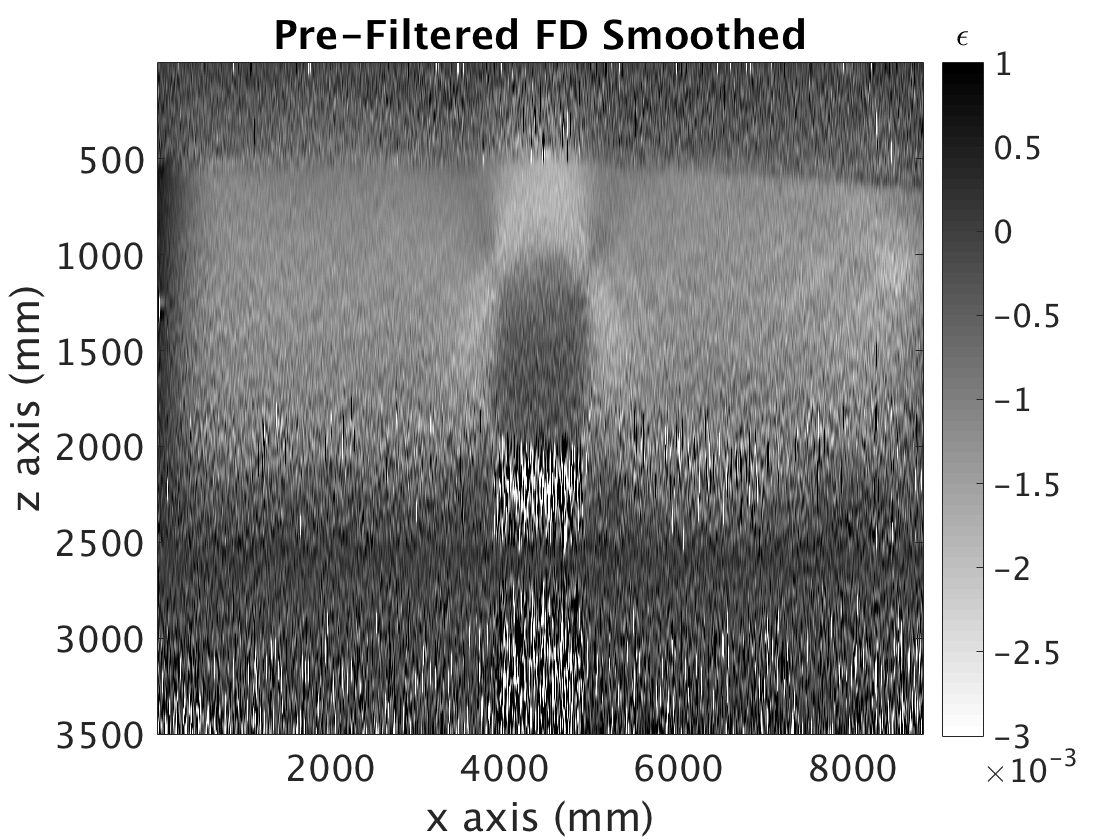
\includegraphics[width=\textwidth]{figures/fdsm_fr70_lr0.png}
    \end{subfigure}
    \caption{Strain B-scans taken from the centre of the phantom for the six strain estimation techniques discussed above. The strain values shown are windowed between -3 and 1 milli-strain.}
    \label{bscan_images_1}	
\end{figure}

\autoref{bscan_images_1} shows the resulting B-scan strain images, taken from the centre of the phantom, for the six different strain estimation techniques described above. Note that negative strain corresponds to compressive force, that is a displacement downwards. The fact that there exist positive strain values suggests that our assumption of uniaxial compression is invalid, as stiffer regions are pushing the softer bulk laterally and upwards. It can seen in all images that the stiff inclusion shows less strain than the softer surrounding bulk, as expected. There are similar 'halo' effects, caused by the stiff inclusion taking more of the compressive force than the soft bulk immediately next to it, in all images. The area under the hard inclusion is characterised by low OCT signal, as can be seen in figure \autoref{oct_image}, and is the most prominently noisy in the techniques that utilise a phase unwrapping algorithm over the entire volume, which is highly sensitive to strong fluctuations in OCT signal and as a result creates artefacts in these regions. A similar pattern is seen in this region in the weighted and unweighted smoothing of FD strain, and is very significant in the pre-filter FD image, which has in addition further streaks of strain estimation arguments at the bottom of the image. 

As mentioned before, the pre-filter FD with smoothed strain algorithm was introduced after noticing significant 'ripple' effects in the weighted smoothing of FD algorithm. These can be seen prominently to the top right of the inclusion, and match with features in the OCT image in \autoref{oct_image}. In addition to this, the surface of the sample, which has a high reflectance and therefore strong optical weighting, is a  prominent artefact in the weighted smoothing FD image. The application of a small pre-filter to this prior to smoothing appears to have removed this issue, as well as slightly decreased the impact of the optical features at the top right, however at the expense of introducing a multitude of streak artefacts into the bottom half of the image in areas of low OCT signal.

\subsection{Processing Time}

\autoref{process_time_1} shows the relative processing time for the different strain estimation techniques for both a single @D B-scan and an entire 3D C-scan, at different fit resolutions. Note that in order to compare accurately between the 2D B-scan and C-scan, a 2D unwrapping algorithm was implemented instead of the usual 3D that laterally unwraps as well. Each data point corresponds to an average of 50 processing time measurements. The error bars in the plot are the standard deviations of these 50 measurements. Since this is plotted relatively, the standard deviation of the relative measurement is equal to the addition of the standard deviations of the absolute measurement and the baseline (WLS) measurement.

The relative processing time (with respect to the WLS with unwrapped phase) is shown instead of the actual, to try provide an estimate that is comparable across different machines.

\begin{figure}[h!]
	\centering
    \begin{subfigure}{0.49\textwidth}
    	\centering
        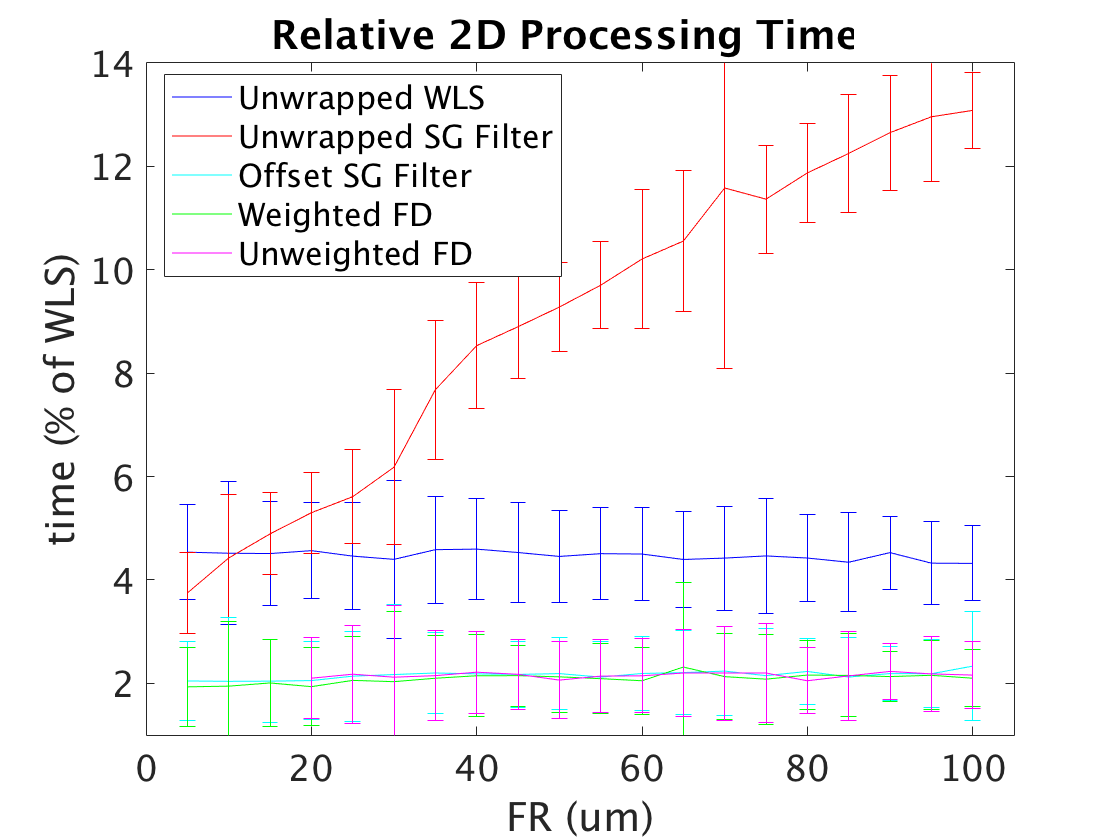
\includegraphics[width=\textwidth]{figures/2d_relative_fr.png}
    \end{subfigure}
    \begin{subfigure}{0.49\textwidth}
    	\centering
        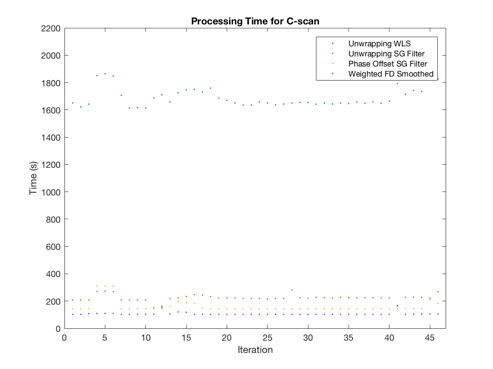
\includegraphics[width=\textwidth]{figures/3d_time_2.png}
    \end{subfigure}
    \caption{Relative processing time for different strain estimation techniques at different fit resolution values for a) a single B-scan and b) an entire C-scan. Error bars are the standard deviation of 50 repeated measurements.}
    \label{process_time_1}
\end{figure}


It can be seen that all new strain estimation techniques show a significant improvement in processing speed compared to the WLS estimate. In particularly, the finite difference techniques are particularly fast. The Savitzky-Golay filter on the unwrapped phase is faster than when applied to the phase offset, suggesting that the bottleneck caused by the non-linear subtraction operation contributes more to slowing the process down than needing to perform unwrapping on the entire volume. 

\subsection{Sensitivity}

\begin{figure}[b!]
	\centering
    \begin{subfigure}{0.49\textwidth}
    	\centering
        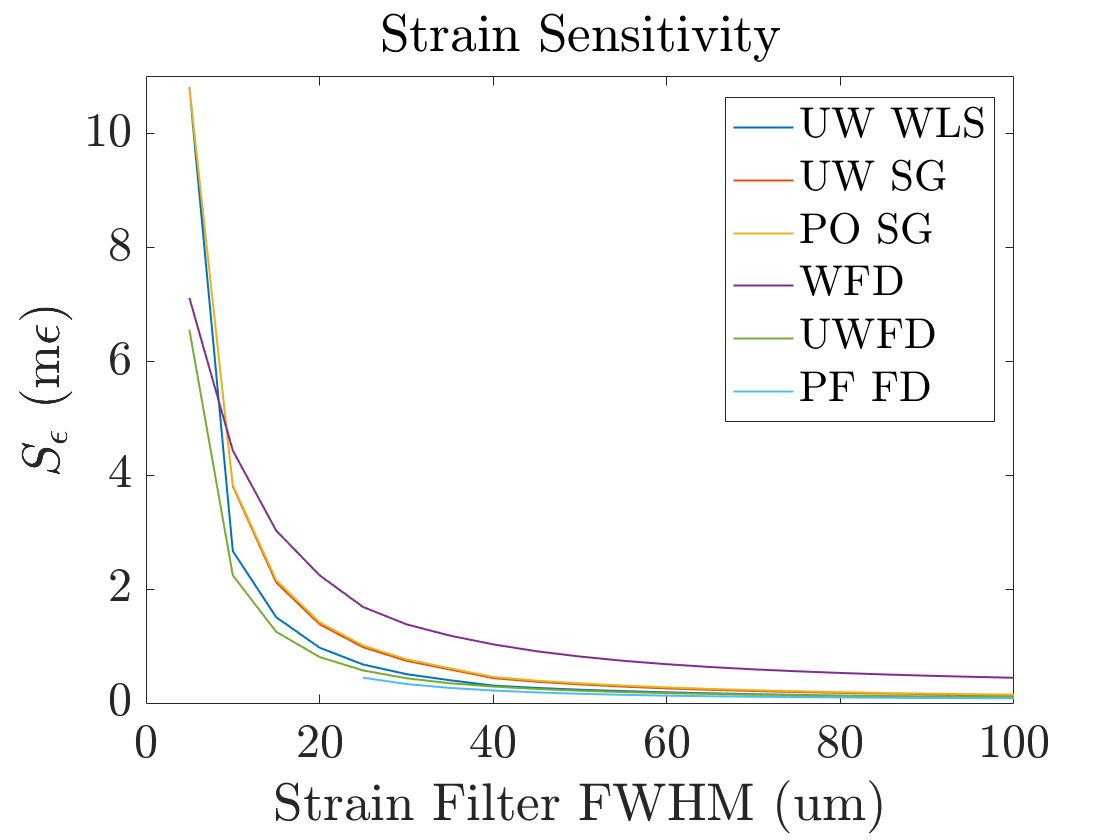
\includegraphics[width=\textwidth]{figures/sensitivity_lr0.png}
    \end{subfigure}
    \begin{subfigure}{0.49\textwidth}
    	\centering
        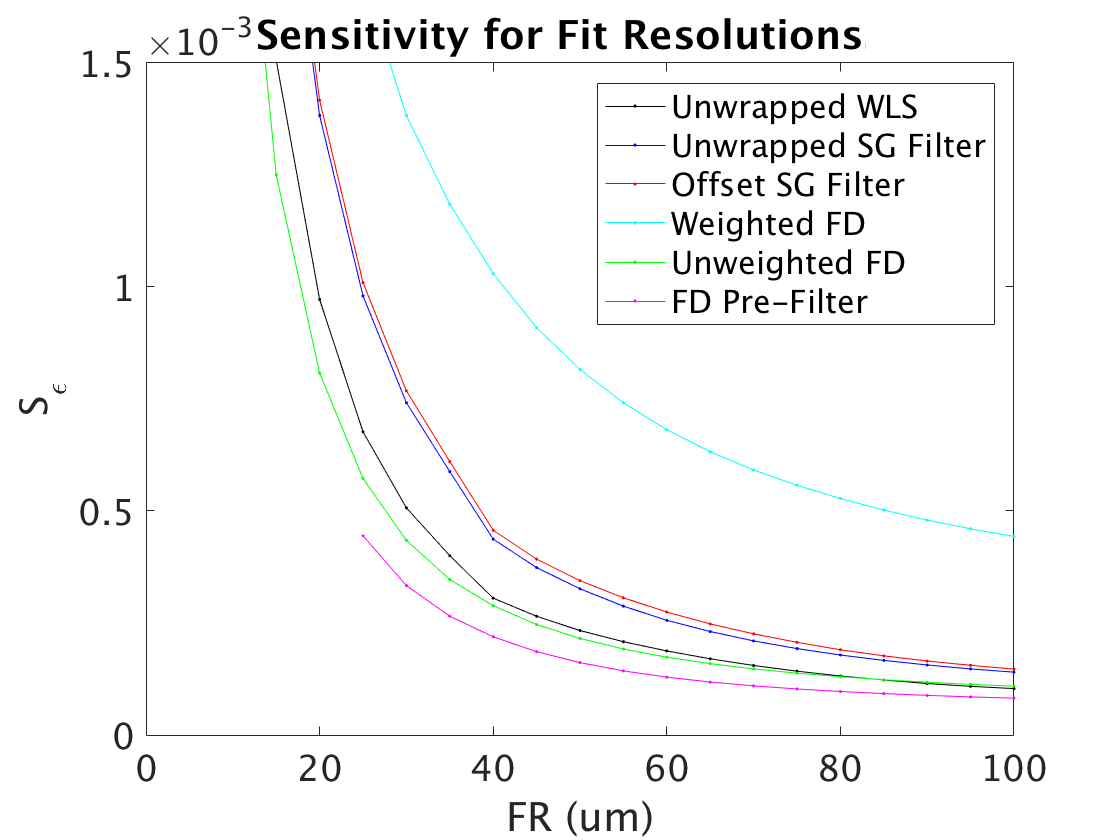
\includegraphics[width=\textwidth]{figures/sensitivity_lr0_zoom.png}
    \end{subfigure}
    \caption{Strain sensitivity values at different fit resolutions for all strain estimation techniques. The plot on the left is zoomed in to show more clearly the differences in behaviour.}
	\label{sensitivity_1}
\end{figure}

The strain sensitivity for the six different estimation techniques for different fit resolutions is shown in Figure \autoref{sensitivity_1}. There is a clear trend across all techniques, that at the larger fit resolutions the sensitivity is better. The downside of this is that at larger fit resolutions, the ability to distinguish objects laterally is significantly worsened, as can be seen in strain B-scan images in \autoref{strain_bscan_images}. Therefore there is a need to optimise the trade off between sensitivity and fit resolution. The three techniques that offer the best sensitivity at lower fit resolutions are WLS, unweighted smoothing with FD, and the pre-filtered FD. Note that the weighted smoothing with FD is significantly worse than the other techniques, due to the artefacts discussed above. The phase offset and unwrapping with SG filtering are slightly worse than the WLS estimate, likely due to them being an ordinary least squares estimate, as opposed to a weighted one.

Although the pre-filtered FD supposedly shows the best sensitivity, it is important to note the artefacts present in the qualitative evaluation of the image. Therefore this sensitivity measurement is not indicative of the image quality as a whole, but only a segment of it.

On the basis of these results, it was decided to see if implementing lateral averaging over the separated B-scans could improve the sensitivity of the lower-order differentiation techniques (in particular the weighted FD and the SG filtering) towards that of the WLS. 

\section{Phantom Strain Elastogram Results with Lateral Averaging}\label{phantom_results_lateral}

\subsection{Qualitative Comparison}
It was found that very comparable image quality could be achieved using a smaller fit resolution of $40\mu m$ when lateral smoothing was also applied. \autoref{images} contains the B-scan  images for the different strain estimation techniques for selected fit resolution and lateral resolution values. 

\subsection{Processing Time}
The benefit of adding lateral averaging is that it improves the sensitivity, and in most instances, without adding much time overhead, since it can be implemented as a 2D convolution on a given B-scan. Therefore the focus of this section is mostly on the image quality, rather than the processing time. However, \autoref{process_time_2} shows that adding lateral smoothing did not change the relative positions of the processing techniques in terms of processing time.

\begin{figure}[th!]
	\centering
    \begin{subfigure}{0.49\textwidth}
    	\centering
        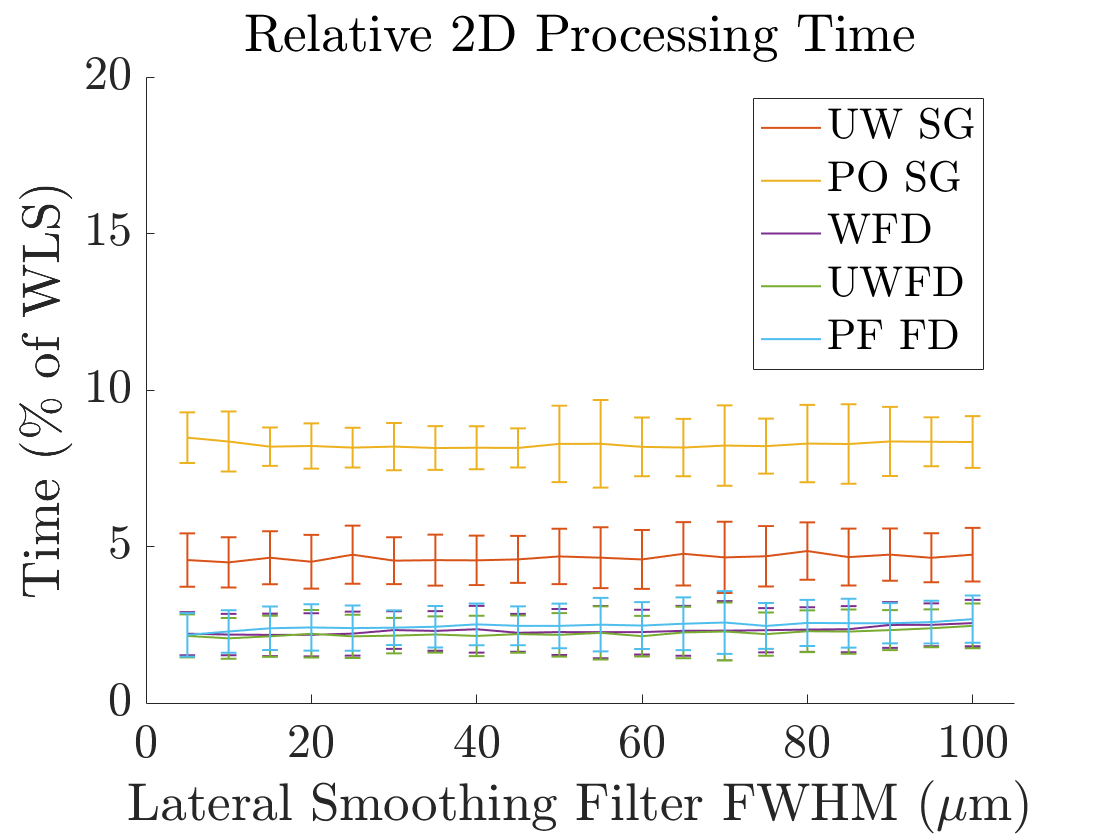
\includegraphics[width=\textwidth]{figures/2d_relative_lr.png}
    \end{subfigure}
    \begin{subfigure}{0.49\textwidth}
    	\centering
        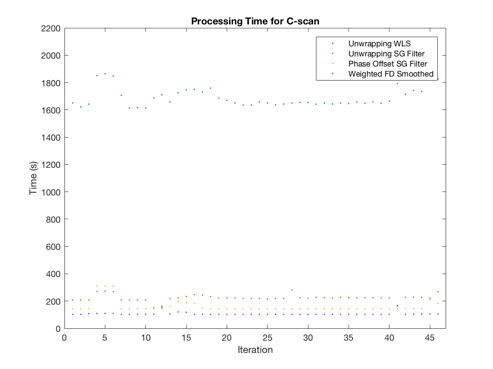
\includegraphics[width=\textwidth]{figures/3d_time_1.png}
    \end{subfigure}
    \caption{Relative processing time for different strain estimation techniques at a fit resolution of $40\mu m$ and with different lateral smoothing resolutions for a) a single B-scan and b) an entire C-scan.}
    \label{process_time_2}
\end{figure}

\subsection{Sensitivity}

\begin{figure}
	\centering
    \begin{subfigure}{0.49\textwidth}
    	\centering
        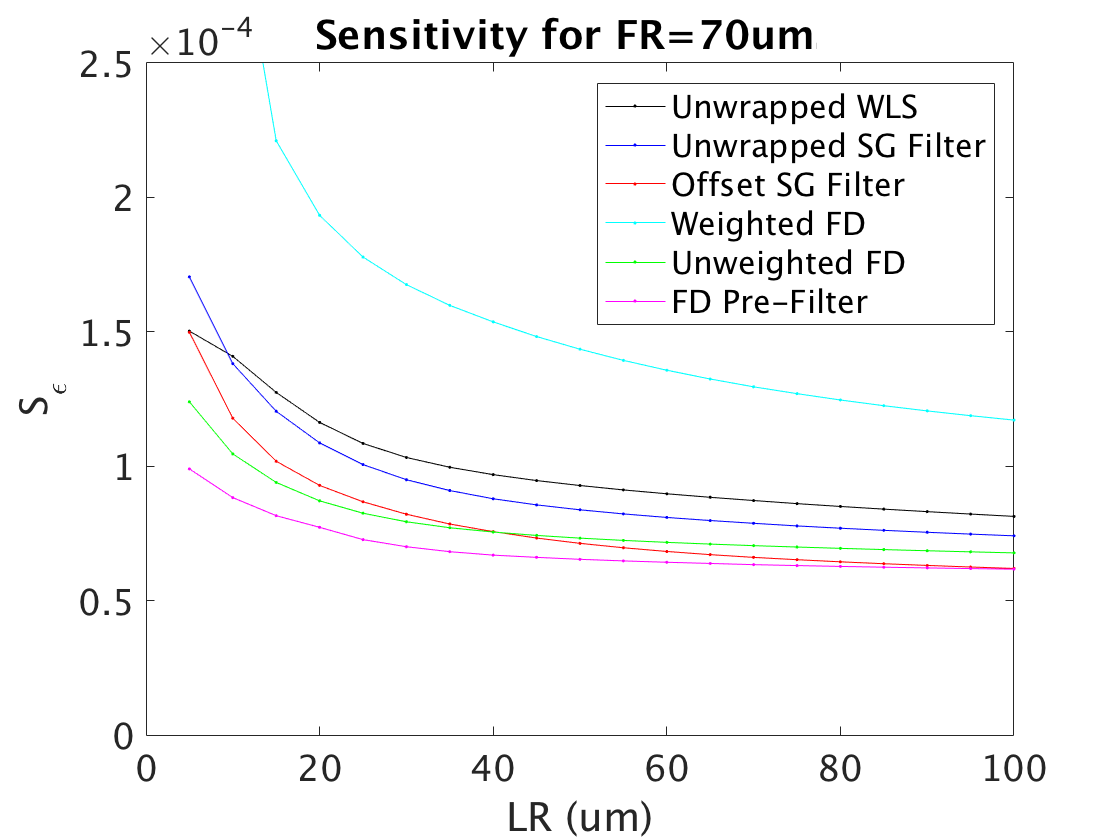
\includegraphics[width=\textwidth]{figures/sensitivity_FR70.png}
    \end{subfigure}
    \begin{subfigure}{0.49\textwidth}
    	\centering
        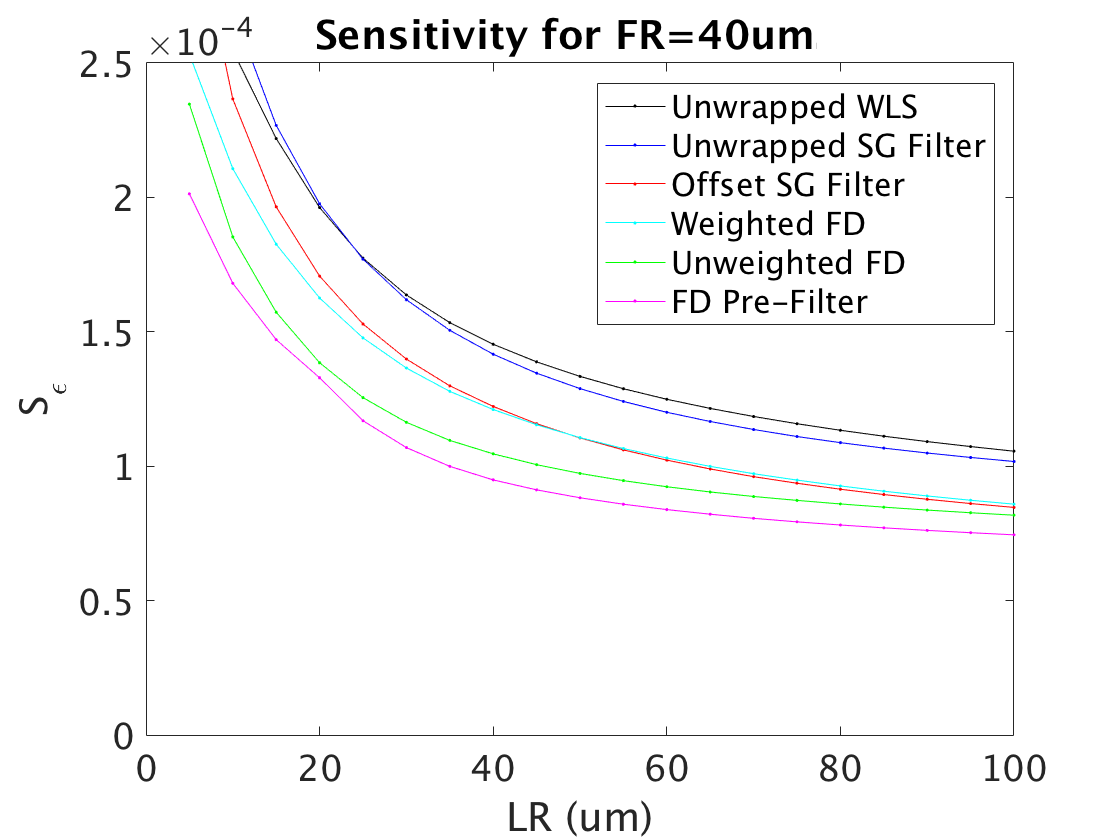
\includegraphics[width=\textwidth]{figures/sensitivity_FR40.png}
    \end{subfigure}
    \caption{Strain sensitivity for different lateral smoothing resolutions for a) Fit resolution of $70\mu m$, and b) $40\mu m$.}
    \label{sensitivity_2}	
\end{figure}

The addition of lateral smoothing heightens the sensitivity of all imaging techniques. At the standard fit resolution, \autoref{sensitivity_2} shows significant improvement in the sensitivity when lateral smoothing is applied, for all techniques.

\begin{table}[h]
	\begin{center}
		\begin{tabular}{|c||c||c|c|c|c|c|c|}
			\hline 
			FR ($\mu m$) & LR ($\mu m$) & WLS & UW SG & PO SG & W FD & UW FD & PF FD \\
			\hline
			\hline
			40 & 0 & 0.3198 & 0.4372 & 0.4571 & 0.2869 & 0.2886 & 0.2192 \\
			\hline
			70 & 0 & 0.1607 & 0.2559 & 0.2744 & 0.2148 & 0.1737 & 0.1291 \\
			\hline
			100 & 0 & 0.1072 & 0.1403 & 0.1469 & 0.1714 & 0.1090 & 0.0821 \\
			\hline
			40 & 20 & 0.1962 & 0.1976 & 0.1707 & 0.1626 & 0.1385 & 0.1329 \\
			\hline
			70 & 20 & 0.1076 & 0.1091 & 0.0961 & 0.1246 & 0.0875 & 0.0793 \\
			\hline
			100 & 20 & 0.0789 & 0.0878 & 0.0710 & 0.1067 & 0.0771 & 0.0685 \\
			\hline
			40 & 40 & 0.1453 & 0.1417 & 0.1222 & 0.1211 & 0.1046 & 0.0949 \\
			\hline
			70 & 40 & 0.0890 & 0.0882 & 0.0770 & 0.0955 & 0.0757 & 0.0678 \\
			\hline
			100 & 40 & 0.0685 & 0.0772 & 0.0593 & 0.0813 & 0.0709 & 0.0632 \\
			\hline
		\end{tabular}
	\end{center}
	\caption{Strain sensitivity values (given in millistrain) for selected fit and lateral resolutions. The six strain estimation techniques are ordered as defined above in \autoref{algorithms}.}
	\label{sensitivity_table}
\end{table}

\autoref{sensitivity_table} shows the sensitivity results for selected combinations of fit and lateral resolutions, for which the images themselves are shown in \autoref{images}.

It has been shown that it is possible to greatly reduce the processing time by using finite difference approaches, and that the sensitivity can be optimised by introducing lateral smoothing, which can be computed very quickly using a convolution operation. However, the image is not infinitely improved with more lateral smoothing and higher fit resolutions. The degradation of the image resolution, due to these processes, must be examined. 

\section{Analysis of Image Resolution} \label{image_res_results}
It was found that the process of fitting a step response to the object boundaries was impossible for strain elastograms with no lateral averaging, due to the high frequency noise corrupting the data. The three 'best' strain estimation techniques were picked based on the results for processing speed and sensitivity in the previous section: unweighted smoothing FD, pre-filtered FD with smoothing, and the unwrapping with SG filtering. The lateral image resolution was plotted for each of these techniques at different lateral resolutions, and for specific fit resolutions ($40\mu m, 70 \mu m, 100\mu m$) in \autoref{lateral_image_res}. The axial image resolution was similarly plotted against the fit resolution, for different values of lateral smoothing: $20\mu m, 40\mu m$, and $70\mu m$ in \autoref{axial_image_res}.

\chapter{Discussion}

Due to the smart scanning patterns, phase-sensitive compression OCE systems are capable of scanning a 3D volume in under 2 seconds. From here, the raw spectral data is 

\section{Optimal Processing Algorithm}

\section{Further Computational Speed Ups}

\begin{itemize}
\item Parallel capabilities of independent looping operations (e.g. any without lateral unwrapping)
\item Convolution on GPUs (need to develop a matlab interface)
\end{itemize}

\section{Next Step}

\begin{itemize}
\item Specificity and sensitivity of diagnosis in breast tissue
\item Quantitative measurements of elasticity
\item Maintaining image quality with removal of B-scan averaging to decrease acquisition time
\end{itemize}


%\newpage
%---------------------------------------------------------
\renewcommand{\bibname}{References}
\bibliography{refs}
\bibliographystyle{styles/hplain}   
%\bibliographystyle{authordate1}
\addcontentsline{toc}{part}{References}
%---------------------------------------------------------

% Appendices
\appendix
\chapter{Riemannian Geometry}


%\chapter{Derivation of Savitzky-Golay Coefficients}

The Savitzky-Golay coefficients are derived from the normal equations in Appendix 1 that describe the least squares estimation procedure.

\chapter{Research Proposal}

This appendix details significant changes that exist between this thesis and the initial research proposal submitted in Semester 1.

The following table lists the changes made to the project in regards to the initial research proposal. The area of interest remained the same: namely, optimising strain estimation methods for use in the assessment of surgical margins in breast conserving surgery. However, the paradigm shift that occurred was from attempting to improve upon the image quality, to attempting to improve the speed at which the image could be produced. Therefore this thesis is structured to first look at speeding up the strain estimation process as much as possible, to enable real-time imaging, and only when that was achieved was the analysis of image quality returned to. 
\begin{itemize}
\item Focus on mechanical noise: 
\end{itemize}

\includepdf[pages=-]{Emily_Hackett_Research_Proposal.pdf}

%---------------------------------------------------------

\end{document}


